\documentclass[12pt, oneside, a4paper]{article}

\usepackage[left=2.5cm, top=2.5cm, bottom=2.5cm, right=2.5cm]{geometry}

\usepackage[utf8]{inputenc}
\usepackage[T1]{polski}
\usepackage[polish]{babel}
\usepackage[]{amsmath}
\usepackage[]{listings}
\usepackage[]{pgf}
\usepackage[]{float}
\usepackage[]{graphics}
\usepackage[]{svg}
\usepackage{booktabs}
\usepackage[tablename=Tabela,margin=0.03\linewidth]{caption}
\usepackage[]{enumitem}
\usepackage{indentfirst}
\usepackage{textcomp}
\usepackage{pdfpages}

\usepackage[hidelinks]{hyperref}
\hypersetup{
    colorlinks=false,
    urlcolor=magenta,
}

\urlstyle{same}


% temporarily for dark background
\usepackage{xcolor}
\definecolor{mybackground}{rgb}{0.15, 0.15, 0.13}
\definecolor{mytext}{rgb}{0.94, 0.94, 0.92}
% \pagecolor{mybackground}
% \color{mytext}

\usepackage[
  color=orange!30,
  textcolor=black,
  figcolor=white,
  figwidth=10cm
]{todonotes}


\lstset{
  basicstyle=\ttfamily,
  captionpos=b,
  aboveskip=2em,
}

% listing settings
\renewcommand{\ttdefault}{pcr}
\lstdefinestyle{hls}{
  language=C++,
  keywordstyle=\ttfamily\bfseries,
  numbers=left,
  numberstyle=\small,
  xleftmargin=2em,
}

\newenvironment{changemargin}[2]{%
\begin{list}{}{%
\setlength{\topsep}{0pt}%
\setlength{\topmargin}{#1}%
% \setlength{\bottommargin}{#2}%
\setlength{\listparindent}{\parindent}%
\setlength{\itemindent}{\parindent}%
\setlength{\parsep}{\parskip}%
}%
\item[]}{\end{list}}

\def\CPP{{C\nolinebreak[4]\hspace{-.05em}\raisebox{.4ex}{\tiny\bf ++}}}
\def\ok{\(\sim \)}

\begin{document}
\thispagestyle{empty}
\begin{titlepage}
    \begin{center}

      \Large
      \textbf{Uniwersytet Jagielloński w~Krakowie}\vspace{0.2cm}\\
        Wydział Fizyki, Astronomii i~Informatyki Stosowanej
      \vspace*{1cm}
               
      \vspace{3cm}
      \Large
      \textbf{Wojciech Lepich}\\\vspace{0.5cm}
      \normalsize Nr albumu: 1146600\\
      \vspace{2cm}
      \Huge
      \textbf{Rozpoznawanie cyfr przez sieć neuronową
      zaimplementowaną na układzie FPGA}
      
      \vspace{1.5cm}
      \normalsize
      Praca licencjacka\\
      na kierunku Informatyka\\ \vspace{0.15cm}
        
      \vfill
      \vspace{2cm}
      \begin{minipage}{1\textwidth}
\begin{flushright}
Praca wykonana pod kierunkiem\\
dr. Grzegorza Korcyla\\
z Zakładu Technologii Informatycznych
\end{flushright}
\end{minipage}
        
        \vspace{2cm}
        \begin{center}
      Kraków 2020
        \end{center}
    \end{center}
\end{titlepage}

\newpage 
\thispagestyle{empty}
\vspace{2.5cm}
\begin{flushleft}
\large \textbf{Oświadczenie autora pracy}\vspace{0.6cm}\\
\end{flushleft}

\noindent Świadom odpowiedzialności prawnej oświadczam, że niniejsza praca
dyplomowa została napisana przeze mnie samodzielnie i~nie zawiera treści
uzyskanych w~sposób niezgodny z~obowiązującymi przepisami.\\

\noindent Oświadczam również, że przedstawiona praca nie była wcześniej
przedmiotem procedur związanych z~uzyskaniem
tytułu zawodowego w~wyższej uczelni.
\vspace{2cm}
\begin{center}
\begin{tabular}{lr}
\ldots\ldots\ldots\ldots\ldots\ldots~~~~~~~~~~~~~~~~~~~~~~~~~~~~~~~~~~~~~~&
\ldots\ldots\ldots\ldots\ldots\ldots\ldots\ldots\ldots \\
{~~~~Kraków, dnia} & {Podpis autora pracy~~~~}
\end{tabular}
\end{center}
\vspace{5cm}
\begin{flushleft}
\large \textbf{Oświadczenie kierującego pracą}
\end{flushleft}

\noindent Potwierdzam, że niniejsza praca została przygotowana pod moim
kierunkiem i~kwalifikuje się do przedstawienia jej w~postępowaniu
o~nadanie tytułu zawodowego.
\vspace{2cm}
\begin{center}
\begin{tabular}{lr}
\ldots\ldots\ldots\ldots\ldots\ldots~~~~~~~~~~~~~~~~~~~~~~~~~~~~~~~~~~~~~~&
\ldots\ldots\ldots\ldots\ldots\ldots\ldots\ldots\ldots \\
{~~~~Kraków, dnia} & {Podpis kierującego pracą~~}
\end{tabular}
\end{center}
\vfill

\newpage
\tableofcontents

\newgeometry{top=5cm, left=2.5cm, right=2.5cm}
\newpage
\section*{Wstęp}
\addcontentsline{toc}{section}{Wstęp}%
Wraz z~intensywnym w~ostatnich latach rozwojem dziedziny nauczania maszynowego,
w~przemyśle komputerowym na dobre zagościło rozpoznawanie obrazów. Stało
się to możliwe dzięki nieustającemu postępowi technologicznemu oraz
dostępowi do coraz większej ilości zasobów komputerowych. Nowe architektury
sieci neuronowych rosną do niewyobrażalnych kilkadziesiąt lat temu rozmiarów.
Przy ciągle rosnącej ilości danych potrzebnych do przetworzenia w~czasie
rzeczywistym, konieczne jest zastosowanie specjalistycznego sprzętu.
Potencjał drzemiący w~układach FPGA w~postaci
ogromnego zrównoleglenia obliczeń, którego nie są w~stanie zaoferować układy CPU,
elastyczności, której nie dają układy ASIC oraz
niskich opóźnień, których nie da się osiągnąć programując układy GPU,
można wykorzystać budując odpowiednio przygotowany model sieci.

W niniejszej pracy zaimplementowano na FPGA model sieci neuronowej rozpoznającej
cyfry. Przygotowano również część odpowiedzialną za wstępne przygotowanie
obrazu z~kamery i~wyświetlającej go na monitorze oraz tej przedstawiającej
wyniki na terminalu komputera.

Praca składa się ze wstępu, trzech rozdziałów podsumowania oraz bibliografii.

W rozdziale pierwszym przedstawione są zagadnienia teoretyczne dotyczące
projektu, potrzebne dla zrozumienia reszty pracy. Znajdują się tam opis
architektury FPGA, problematyka przetwarzania obrazów oraz krótki wstęp
do rozległego tematu sieci neuronowych.

Rozdział drugi to przedstawienie projektu zaczynając od opisu
sprzętu oraz wykorzystanych narzędzi, następnie wyjaśnione zostają kroki
czynione w~trakcie tworzenia projektu, na koniec przedstawiono informacje
dotyczące uruchamiania.

Ostatni rozdział zawiera wyniki predykcji sieci wraz z~dyskusją co wpływa
na te osiągnięte oraz na jakie sposoby można potencjalnie uzyskać ich poprawę.

Na zakończenie składam serdeczne podziękowania dr. Grzegorzowi Korcylowi
za pomoc w~nakreśleniu projektu oraz cenne uwagi podczas pisania pracy.
\restoregeometry{}

\newpage
\section{Teoria}\label{sec:Teoria}
\subsection{Architektura FPGA}\label{sec:Architektura FPGA}
Field-Programmable Gate Array (FPGA) to układy scalone, które mogą być
elektronicznie przeprogramowane bez potrzeby demontażu samego układu
z urządzenia. W~porównaniu do układów ASIC znacznie taniej zaprojektować
pierwszy działający układ. Elastyczna natura układów FPGA wiąże się z~większym
zużyciem powierzchni krzemu, opóźnień oraz zużycia energii.\cite{kuon08}

Podstawowa struktura układów FPGA składa się z~różnych bloków logicznych,
które mogą być łączone ze sobą w~zależności od wymagań projektowych.
Przykładami takich bloków są:
DSP (jednostka przeprowadzająca obliczenia dodawania/mnożenia),
LUT (Look-Up Table, de facto tablica prawdy dowolnej funkcji boolowskiej),
Flip Flop (przechowują wynik LUT), BRAM (Block RAM, pamięć dwuportowa,
jest w~stanie przechowywać względnie dużą ilość danych).

Układy FPGA przeważnie pracują na kilku-, kilkunastukrotnie niższych
częstotliwościach niż CPU. Osiągają wysoką wydajność
dzięki masywnemu zrównolegleniu obliczeń.

Programowanie FPGA polega na pisaniu logiki
w językach HDL (Hardware Description Language) takimi jak VHDL 
czy też Verilog. Napisana logika definiuje zachowanie układu FPGA.
Gotowy opis logiki syntetyzuje się, czyli generuje połączenia pomiędzy
zasobami układu. Kolejnym etapem jest implementacja --- odzworowanie
połączeń w~konkretnym układzie.
 
HLS (High-Level Synthesis) to proces ułatwiający pisanie skomplikowanej
logiki. Algorytmy można pisać w~językach wysokiego poziomu, takich jak
C, \CPP, SystemC. Przygotowany kod jest transpilowany poprzez odpowiedni
kompilator HLS do języka RTL (Register-Transfer Level; język opisu sprzętu
na poziomie bramek i~rejestrów), a~ten może być zaimplementowany na układzie.

\subsection{Przetwarzanie obrazu}\label{sec:Przetwarzanie obrazu}
Cyfrowe przetwarzanie obrazu jest problemem wymagającym dużych mocy
obliczeniowych ze względu na ilość danych do przetworzenia. Nieskompresowany
kolorowy obraz z~pikselami w~formacie RGB (po 8 bitów na kolor) o~wysokości
720 pikseli i~szerokości 1280 pikseli to 22118400 bitów (\(\approx \) 2,5MB). Obraz
przetwarzany w~czasie rzeczywistym, na przykład z~kamery, zwielokrotnia tę
liczbę o~liczbę klatek na sekundę (przy trzydziestu klatkach na sekundę liczba
danych rośnie do około 79 megabajtów na sekundę). Należy również pamiętać, że
dane są dwuwymiarowe co jest ważne przy problemach związanych z~rozpoznawaniem
wzorców, klasyfikacją przedmiotów na obrazie, filtrowania w~celu rozmazania lub
wyostrzenia obrazów itp.

\subsubsection{Formaty pikseli}\label{Formaty pikseli}
Jest wiele modeli przestrzeni barw (a co za tym idzie, sposobów kodowania
pikseli) między innymi:
\begin{itemize}
  \setlength\itemsep{0.0em}
  \item RGB, używany w~aparatach, skanerach, telewizorach
  \item CMYK, używany w~druku wielobarwnym
  \item HSV
  \item YUV
\end{itemize}
Składowe dwóch ostatnich przestrzeni barw oddzielają informację o~jasności
od informacji o~kolorach. Model barw YUV składa się z~kanału luminacji~Y
i~kanałów kodujących barwę U oraz V, są to kolejno składowa niebieska
i składowa czerwona. W~projekcie użyty jest format pikseli YUY2 (znany też
pod nazwą YUYV), w~którym na dwa piksele przypadają 32 bity.
Licząc od najstarszego bitu, pierwsze osiem bitów przypada na Y0 (patrz
rys.~\ref{fig:yuv2}), to jest
luminacja pierwszego piksela; następne osiem bitów na U0; kolejne osiem bitów
to luminacja drugiego piksela; pozostałe bity to składowa czerwona V0.
Dla obydwóch pikseli składowe U~i~V są wspólne. Co istotne w~projekcie
łatwo oddzielić luminację, która jest używana w~przetwarzaniu obrazu.
\begin{figure}[h]
  \centering
  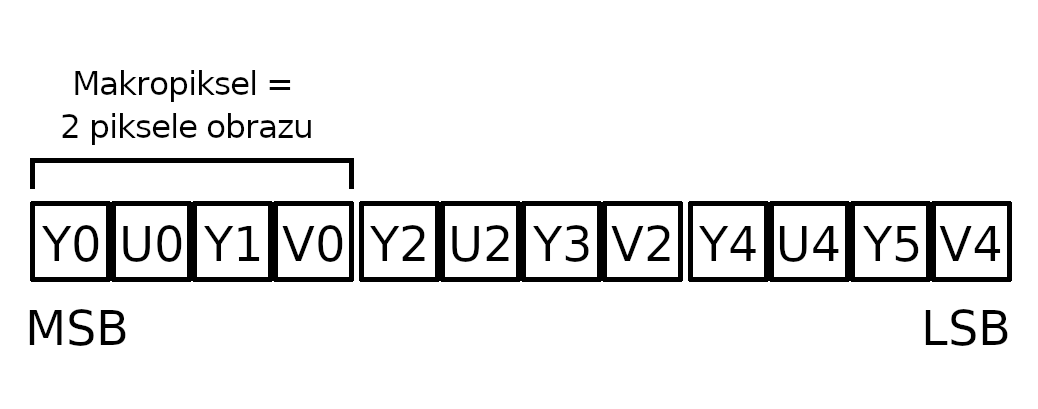
\includegraphics[scale=1.4]{figures/yuv2-scheme.png} 
  \caption{Schemat formatu pikseli YUV2}\label{fig:yuv2}
\end{figure}

\subsection{Sieci neuronowe}\label{sec:Sieci neuronowe}
Sztuczna sieć neuronowa (SSN) jest modelem zdolnym do odwzorowania złożonych
funkcji. Najprostsze sieci są zbudowane ze sztucznych neuronów, z~których każdy
posiada wiele wejść oraz jedno wyjście, które może być połączone z~wejściami
wielu innych neuronów. Każde z~wejść neuronu jest związane ze znalezioną
w procesie trenowania wagą. Wartość wyjścia to obliczony wynik funkcji aktywacji
z sumy ważonych wejść. Sieć może mieć wiele warstw neuronów ukrytych, których
wejściami są wyjścia neuronów z~poprzedniej warstwy. 

Sieci neuronowe są stosowane w~problemach
związanych z~predykcją, klasyfikacją, przetwarzaniem i~analizowaniem
danych. Do ich zastosowania nie jest potrzebna znajomość algorytmu rozwiązania
danego problemu. Obliczenia w~sieciach są wykonywane równolegle w~każdej
warstwie, dzięki czemu implementacja sieci na układzie FPGA może działać
wielokrotnie szybciej niż na CPU, pomimo niższej częstotliwości układu.

\newpage
\section{Opis projektu}\label{sec:Opis projektu}

\subsection{Zarys projektu}\label{sec:Zarys projektu}
Celem projektu jest implementacja systemu do rozpoznawania cyfr
w czasie rzeczywistym. Cel zrealizowano poprzez implementację
wtyczki GStreamera, wykorzystującej sieć neuronową na układzie
Xilinx Zynq MPSoC oraz stworzenie odpowiedniego potoku danych
korzystając z~bibliotek GStreamer. Zadaniami spoczywającymi na innych
elementach potoku jest obsługa kamery,
kadrowanie i~skalowanie obrazu oraz wyświetlenie go na końcowym urządzeniu.

\subsection{Platforma}\label{sec:Platforma}
\begin{figure}[h]
  \centering
  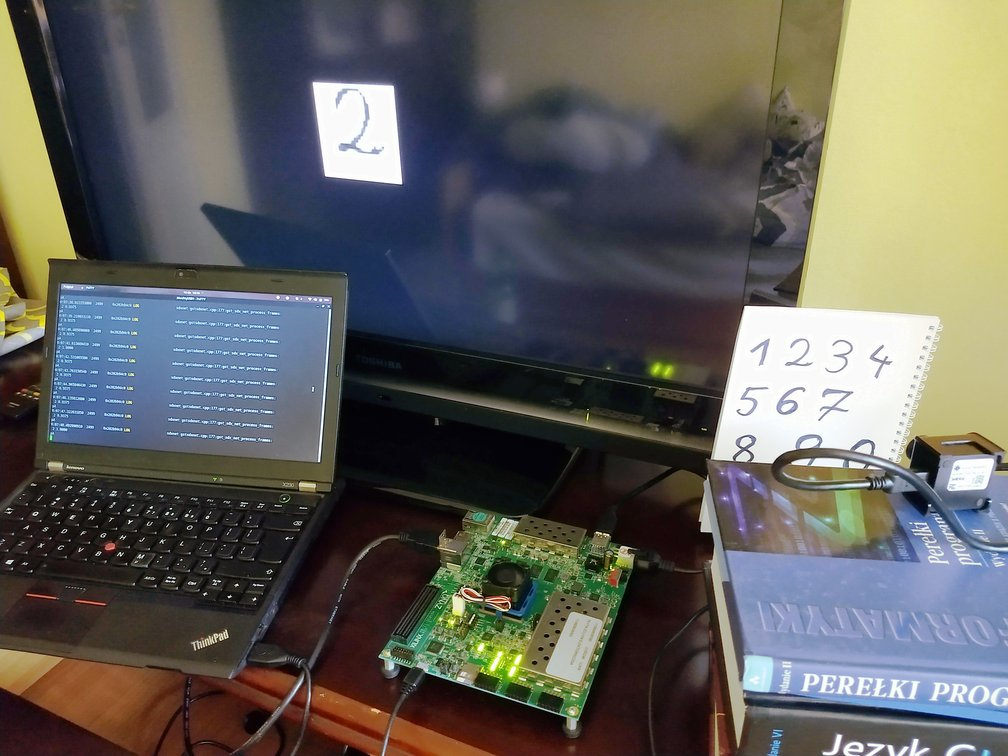
\includegraphics[width=0.9\linewidth]{figures/place_of_work_small.jpg}
  \caption{Stanowisko testowe}\label{fig:stanowisko}
\end{figure}
Sprzęt wykorzystany w~projekcie to Xilinx Zynq UltraScale+ MPSoC ZCU104.
\linebreak
Na jednym układzie znajduje się czterordzeniowy procesor
ARM \mbox{Cortex-A53},
dwurdzeniowy procesor ARM \mbox{Cortex-R5},
układ graficzny \mbox{Mali-400} oraz zasoby FPGA.
Całość projektu została oparta o~platformę Xilinx reVISION\cite{revision}.
Przetwarzane
dane dostarczane są z~kamery USB, która była dołączona w~zestawie z~płytą Zynq.
Urządzeniem końcowym jest telewizor połączony przewodem HDMI z~płytą.

\newpage
\subsection{Sieć neuronowa}\label{sec:Siec neuronowa}
Architektura sieci została dobrana uwzględniając dostępne zasoby programowalnej
logiki na płycie, a~także możliwości sprzętu na którym dokonywana była jej
synteza. Dla problemu klasyfikowania obrazów dobrze nadają się sieci
splotowe (konwolucyjne, ang.\ convolutional neural networks --- CNN), 
których przykładem jest popularna sieć \mbox{LeNet-5}.\cite{lecun98}
Architektura ta zawiera zarówno w~pełni połączone warstwy
oraz warstwy splotowe i~łączące.
Niestety, z~powodu ograniczeń sprzętowych, w~pracy nie została użyta ta
architektura.

Model wykorzystany w~projekcie posiada 2 warstwy ukryte, posiadające kolejno
12 i~40 neuronów aktywowanych funkcją ReLU oraz warstwy wyjściowej złożonej
z 10 neuronów z~funkcją aktywacji softmax.
\begin{figure}[h]
\hspace{2cm}
  \centering
  % 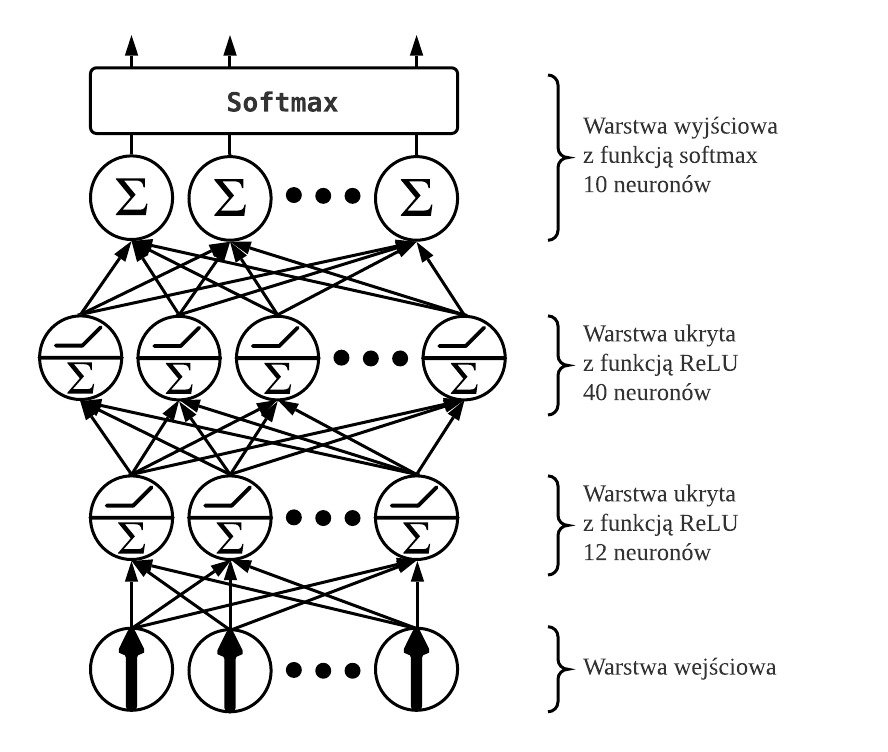
\includegraphics{figures/network-scheme.png}
  \includesvg[scale=0.6]{figures/nn-scheme.svg}
  \caption{Schemat użytej architektury.
  }\label{fig:nn-scheme}
\end{figure}

Do stworzenia sieci wykorzystano
bibliotekę TensorFlow. Sieć uczona była na danych
z bazy MNIST\cite{mnist} składającej się łącznie z~70000 przykładów
cyfr na obrazach o~wielkości 28\(\times \)28 pikseli, z~których każdy
przedstawiony jest jako wartość od 0 (kolor czarny) do 255 (kolor biały).
Próbki zostały
podzielone na zbiór uczący, liczący 60000 próbek, oraz zbiór do testów
z pozostałych 10000 cyfr. Cyfry składają się z białych pikseli, tło jest czarne.
Dokonano prób trenowania sieci przetworzonymi danymi, w~których kolory były
odwrócone, natomiast wytrenowane modele w~trakcie testów nie przekraczały
progu czterdziestu procent dobrze zaklasyfikowanych obrazów.

\newpage
\subsection{hls4ml}\label{sec:hls4ml}
\subsubsection{Idea hls4ml}\label{sec:Idea hls4ml}
Celem projektu hls4ml jest wygenerowanie kodu \CPP{} na podstawie zapisanego
modelu z~TensorFlow. Przykładowy schemat pracy z~hls4ml przedstawiony jest
na rysunku~\ref{fig:hls4ml}.
Czerwona część schematu pokazuje ogólną organizację pracy przy projektowaniu 
odpowiedniego modelu uczenia maszynowego. Niebieska część należy do hls4ml,
który tłumaczy dostarczony model z~wagami do syntetyzowalnego kodu, który
następnie można włączyć do większego projektu lub zaimplementować jako
samodzielną część na FPGA. Generowany projekt jest parametryzowany
przez plik konfiguracyjny yml zawierający ścieżkę do pliku z~zapisanym modelem
wraz z~wagami, typy danych kodujące wartości wag, nazwę docelowego układu FPGA
oraz parametry optymalizacji dotyczące zużycia zasobów --- większa ilość
zasobów oznacza zrównoleglenie większej części obliczeń.
\begin{figure}[h]
  \centering
  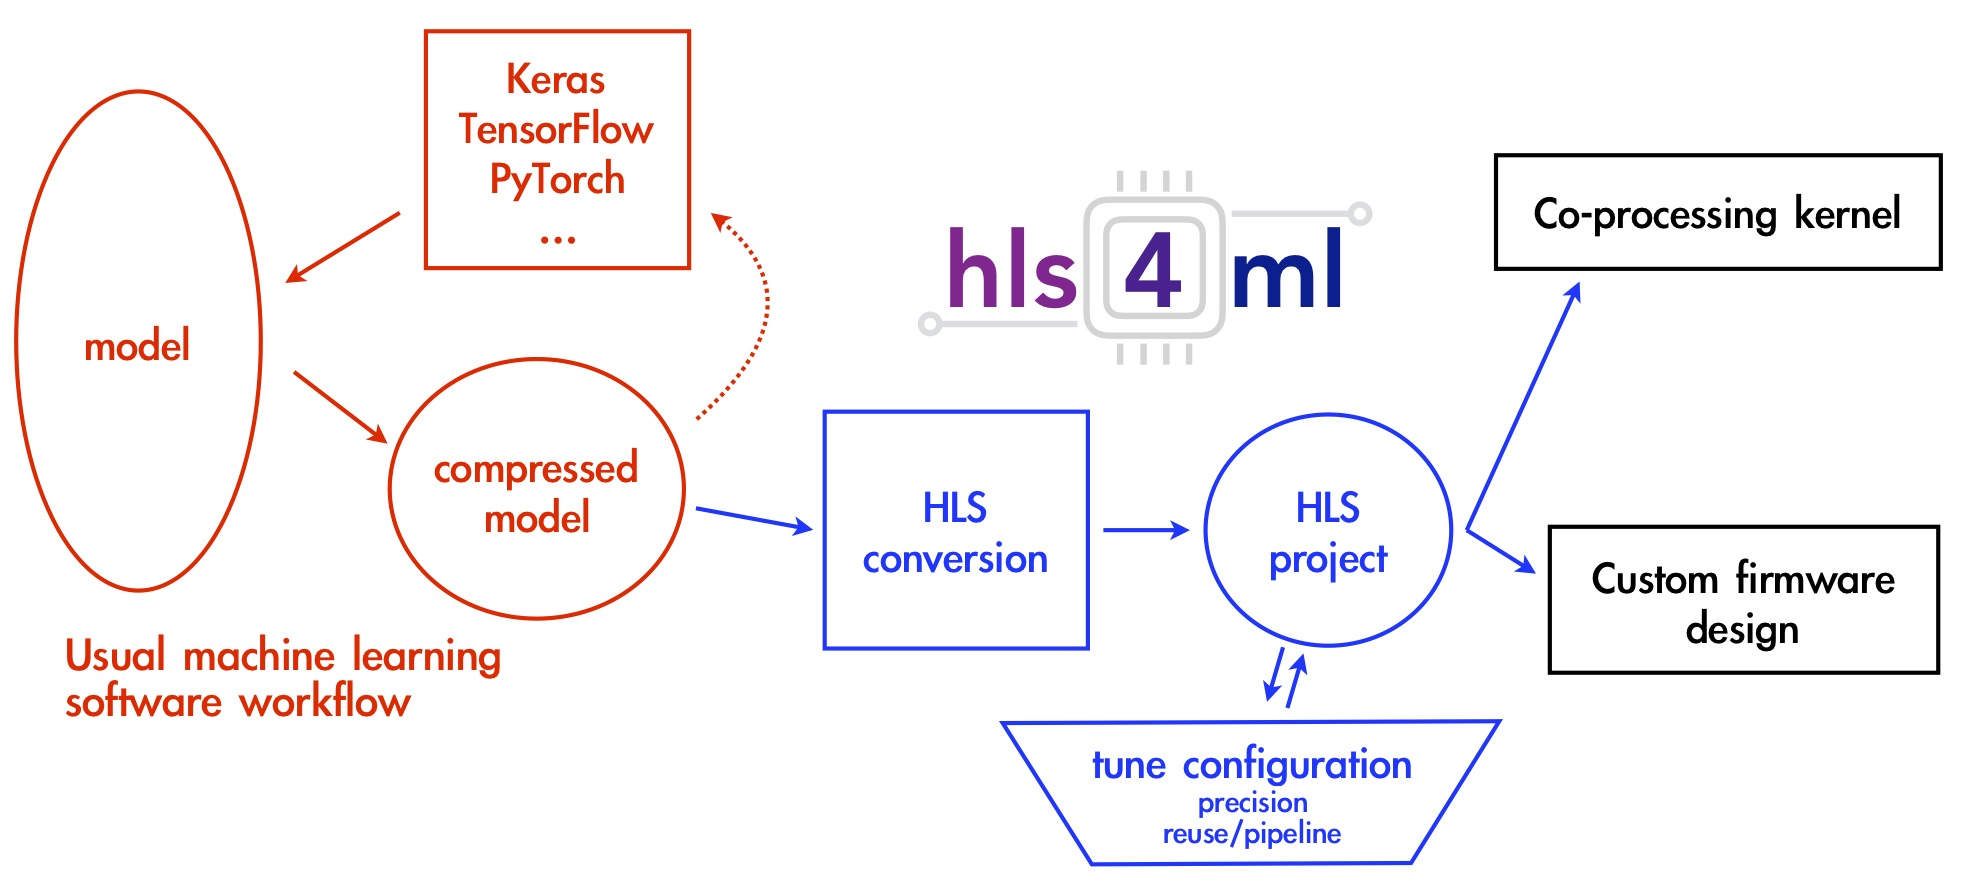
\includegraphics[width=0.95\linewidth]{figures/hls4ml.jpg}
  \caption{Schemat pracy z~hls4ml. \\
  \textit{Dokumentacja hls4ml},
  \url{https://fastmachinelearning.org/hls4ml/CONCEPTS.html}}\label{fig:hls4ml}
\end{figure}

\subsubsection{Precyzja danych}\label{sec:Precyzja danych}
Typ danych używany w~przekonwertowanym modelu to duże liczby
stałoprzecinkowe (\lstinline{ap_fixed}) oraz liczby całkowite
(\lstinline{ap_int}).
Precyzję obu typów można ustalić do jednego bita.
Obliczenia przeprowadzane na liczbach o~mniejszej
precyzji umożliwiają większe zrównoleglenie obliczeń,
natomiast zbyt niska precyzja może poskutkować
bezużytecznością zsyntetyzowanej sieci. Aby odpowiednio dobrać precyzję
wag, skorzystano z~pythonowej biblioteki hls4ml.profiling.

Program korzystający z~funkcji dostarczanych przez tę bibliotekę
analizuje plik konfiguracyjny yml oraz model z~pliku h5.
Wynikiem działania programu jest wykres (patrz rys.~\ref{fig:weights_dist}) przedstawiający
rozkład wartości wag każdej z~warstw modelu otrzymanych w~procesie trenowania.
Szare pole w~tle wykresu
przedstawia zakres wartości, które obejmowane są przez precyzję określoną
w pliku konfiguracyjnym. Dobrym punktem początkowym jest wybranie takiej
liczby bitów dla każdej z~warstw, która obejmuje wszystkie możliwe wagi.
Dalsze ustalanie precyzji można wykonać w~trakcie analizy wyników
symulacji.
\begin{figure}[H]
  \centering
  %% Creator: Matplotlib, PGF backend
%%
%% To include the figure in your LaTeX document, write
%%   \input{<filename>.pgf}
%%
%% Make sure the required packages are loaded in your preamble
%%   \usepackage{pgf}
%%
%% Figures using additional raster images can only be included by \input if
%% they are in the same directory as the main LaTeX file. For loading figures
%% from other directories you can use the `import` package
%%   \usepackage{import}
%% and then include the figures with
%%   \import{<path to file>}{<filename>.pgf}
%%
%% Matplotlib used the following preamble
%%   \usepackage{fontspec}
%%   \setmainfont{DejaVuSerif.ttf}[Path=/home/wojtek/miniconda3/envs/hls4ml_prof/lib/python3.6/site-packages/matplotlib/mpl-data/fonts/ttf/]
%%   \setsansfont{DejaVuSans.ttf}[Path=/home/wojtek/miniconda3/envs/hls4ml_prof/lib/python3.6/site-packages/matplotlib/mpl-data/fonts/ttf/]
%%   \setmonofont{DejaVuSansMono.ttf}[Path=/home/wojtek/miniconda3/envs/hls4ml_prof/lib/python3.6/site-packages/matplotlib/mpl-data/fonts/ttf/]
%%
\begingroup%
\makeatletter%
\begin{pgfpicture}%
\pgfpathrectangle{\pgfpointorigin}{\pgfqpoint{5.400000in}{4.000000in}}%
\pgfusepath{use as bounding box, clip}%
\begin{pgfscope}%
\pgfsetbuttcap%
\pgfsetmiterjoin%
\definecolor{currentfill}{rgb}{1.000000,1.000000,1.000000}%
\pgfsetfillcolor{currentfill}%
\pgfsetlinewidth{0.000000pt}%
\definecolor{currentstroke}{rgb}{1.000000,1.000000,1.000000}%
\pgfsetstrokecolor{currentstroke}%
\pgfsetdash{}{0pt}%
\pgfpathmoveto{\pgfqpoint{0.000000in}{0.000000in}}%
\pgfpathlineto{\pgfqpoint{5.400000in}{0.000000in}}%
\pgfpathlineto{\pgfqpoint{5.400000in}{4.000000in}}%
\pgfpathlineto{\pgfqpoint{0.000000in}{4.000000in}}%
\pgfpathclose%
\pgfusepath{fill}%
\end{pgfscope}%
\begin{pgfscope}%
\pgfsetbuttcap%
\pgfsetmiterjoin%
\definecolor{currentfill}{rgb}{1.000000,1.000000,1.000000}%
\pgfsetfillcolor{currentfill}%
\pgfsetlinewidth{0.000000pt}%
\definecolor{currentstroke}{rgb}{0.000000,0.000000,0.000000}%
\pgfsetstrokecolor{currentstroke}%
\pgfsetstrokeopacity{0.000000}%
\pgfsetdash{}{0pt}%
\pgfpathmoveto{\pgfqpoint{0.808711in}{0.523981in}}%
\pgfpathlineto{\pgfqpoint{5.273438in}{0.523981in}}%
\pgfpathlineto{\pgfqpoint{5.273438in}{3.705556in}}%
\pgfpathlineto{\pgfqpoint{0.808711in}{3.705556in}}%
\pgfpathclose%
\pgfusepath{fill}%
\end{pgfscope}%
\begin{pgfscope}%
\pgfpathrectangle{\pgfqpoint{0.808711in}{0.523981in}}{\pgfqpoint{4.464727in}{3.181574in}}%
\pgfusepath{clip}%
\pgfsetbuttcap%
\pgfsetmiterjoin%
\definecolor{currentfill}{rgb}{0.840692,0.901638,0.958662}%
\pgfsetfillcolor{currentfill}%
\pgfsetlinewidth{1.003750pt}%
\definecolor{currentstroke}{rgb}{0.840692,0.901638,0.958662}%
\pgfsetstrokecolor{currentstroke}%
\pgfsetdash{}{0pt}%
\pgfpathmoveto{\pgfqpoint{3.668229in}{0.683060in}}%
\pgfpathlineto{\pgfqpoint{3.777437in}{0.683060in}}%
\pgfpathlineto{\pgfqpoint{3.777437in}{1.001218in}}%
\pgfpathlineto{\pgfqpoint{3.668229in}{1.001218in}}%
\pgfpathclose%
\pgfusepath{stroke,fill}%
\end{pgfscope}%
\begin{pgfscope}%
\pgfpathrectangle{\pgfqpoint{0.808711in}{0.523981in}}{\pgfqpoint{4.464727in}{3.181574in}}%
\pgfusepath{clip}%
\pgfsetbuttcap%
\pgfsetmiterjoin%
\definecolor{currentfill}{rgb}{0.671895,0.814379,0.900654}%
\pgfsetfillcolor{currentfill}%
\pgfsetlinewidth{1.003750pt}%
\definecolor{currentstroke}{rgb}{0.671895,0.814379,0.900654}%
\pgfsetstrokecolor{currentstroke}%
\pgfsetdash{}{0pt}%
\pgfpathmoveto{\pgfqpoint{3.484240in}{1.319375in}}%
\pgfpathlineto{\pgfqpoint{3.717507in}{1.319375in}}%
\pgfpathlineto{\pgfqpoint{3.717507in}{1.637532in}}%
\pgfpathlineto{\pgfqpoint{3.484240in}{1.637532in}}%
\pgfpathclose%
\pgfusepath{stroke,fill}%
\end{pgfscope}%
\begin{pgfscope}%
\pgfpathrectangle{\pgfqpoint{0.808711in}{0.523981in}}{\pgfqpoint{4.464727in}{3.181574in}}%
\pgfusepath{clip}%
\pgfsetbuttcap%
\pgfsetmiterjoin%
\definecolor{currentfill}{rgb}{0.417086,0.680631,0.838231}%
\pgfsetfillcolor{currentfill}%
\pgfsetlinewidth{1.003750pt}%
\definecolor{currentstroke}{rgb}{0.417086,0.680631,0.838231}%
\pgfsetstrokecolor{currentstroke}%
\pgfsetdash{}{0pt}%
\pgfpathmoveto{\pgfqpoint{3.184987in}{1.955690in}}%
\pgfpathlineto{\pgfqpoint{3.785356in}{1.955690in}}%
\pgfpathlineto{\pgfqpoint{3.785356in}{2.273847in}}%
\pgfpathlineto{\pgfqpoint{3.184987in}{2.273847in}}%
\pgfpathclose%
\pgfusepath{stroke,fill}%
\end{pgfscope}%
\begin{pgfscope}%
\pgfpathrectangle{\pgfqpoint{0.808711in}{0.523981in}}{\pgfqpoint{4.464727in}{3.181574in}}%
\pgfusepath{clip}%
\pgfsetbuttcap%
\pgfsetmiterjoin%
\definecolor{currentfill}{rgb}{0.215686,0.529412,0.754248}%
\pgfsetfillcolor{currentfill}%
\pgfsetlinewidth{1.003750pt}%
\definecolor{currentstroke}{rgb}{0.215686,0.529412,0.754248}%
\pgfsetstrokecolor{currentstroke}%
\pgfsetdash{}{0pt}%
\pgfpathmoveto{\pgfqpoint{3.444094in}{2.592005in}}%
\pgfpathlineto{\pgfqpoint{3.788213in}{2.592005in}}%
\pgfpathlineto{\pgfqpoint{3.788213in}{2.910162in}}%
\pgfpathlineto{\pgfqpoint{3.444094in}{2.910162in}}%
\pgfpathclose%
\pgfusepath{stroke,fill}%
\end{pgfscope}%
\begin{pgfscope}%
\pgfpathrectangle{\pgfqpoint{0.808711in}{0.523981in}}{\pgfqpoint{4.464727in}{3.181574in}}%
\pgfusepath{clip}%
\pgfsetbuttcap%
\pgfsetmiterjoin%
\definecolor{currentfill}{rgb}{0.062514,0.357509,0.642907}%
\pgfsetfillcolor{currentfill}%
\pgfsetlinewidth{1.003750pt}%
\definecolor{currentstroke}{rgb}{0.062514,0.357509,0.642907}%
\pgfsetstrokecolor{currentstroke}%
\pgfsetdash{}{0pt}%
\pgfpathmoveto{\pgfqpoint{3.360485in}{3.228319in}}%
\pgfpathlineto{\pgfqpoint{3.656129in}{3.228319in}}%
\pgfpathlineto{\pgfqpoint{3.656129in}{3.546477in}}%
\pgfpathlineto{\pgfqpoint{3.360485in}{3.546477in}}%
\pgfpathclose%
\pgfusepath{stroke,fill}%
\end{pgfscope}%
\begin{pgfscope}%
\pgfpathrectangle{\pgfqpoint{0.808711in}{0.523981in}}{\pgfqpoint{4.464727in}{3.181574in}}%
\pgfusepath{clip}%
\pgfsetbuttcap%
\pgfsetmiterjoin%
\definecolor{currentfill}{rgb}{0.501961,0.501961,0.501961}%
\pgfsetfillcolor{currentfill}%
\pgfsetfillopacity{0.200000}%
\pgfsetlinewidth{1.003750pt}%
\definecolor{currentstroke}{rgb}{0.501961,0.501961,0.501961}%
\pgfsetstrokecolor{currentstroke}%
\pgfsetstrokeopacity{0.200000}%
\pgfsetdash{}{0pt}%
\pgfpathmoveto{\pgfqpoint{0.917817in}{3.132872in}}%
\pgfpathlineto{\pgfqpoint{4.323132in}{3.132872in}}%
\pgfpathlineto{\pgfqpoint{4.323132in}{3.641924in}}%
\pgfpathlineto{\pgfqpoint{0.917817in}{3.641924in}}%
\pgfpathclose%
\pgfusepath{stroke,fill}%
\end{pgfscope}%
\begin{pgfscope}%
\pgfpathrectangle{\pgfqpoint{0.808711in}{0.523981in}}{\pgfqpoint{4.464727in}{3.181574in}}%
\pgfusepath{clip}%
\pgfsetbuttcap%
\pgfsetmiterjoin%
\definecolor{currentfill}{rgb}{0.501961,0.501961,0.501961}%
\pgfsetfillcolor{currentfill}%
\pgfsetfillopacity{0.200000}%
\pgfsetlinewidth{1.003750pt}%
\definecolor{currentstroke}{rgb}{0.501961,0.501961,0.501961}%
\pgfsetstrokecolor{currentstroke}%
\pgfsetstrokeopacity{0.200000}%
\pgfsetdash{}{0pt}%
\pgfpathmoveto{\pgfqpoint{0.917817in}{2.496557in}}%
\pgfpathlineto{\pgfqpoint{4.323132in}{2.496557in}}%
\pgfpathlineto{\pgfqpoint{4.323132in}{3.005609in}}%
\pgfpathlineto{\pgfqpoint{0.917817in}{3.005609in}}%
\pgfpathclose%
\pgfusepath{stroke,fill}%
\end{pgfscope}%
\begin{pgfscope}%
\pgfpathrectangle{\pgfqpoint{0.808711in}{0.523981in}}{\pgfqpoint{4.464727in}{3.181574in}}%
\pgfusepath{clip}%
\pgfsetbuttcap%
\pgfsetmiterjoin%
\definecolor{currentfill}{rgb}{0.501961,0.501961,0.501961}%
\pgfsetfillcolor{currentfill}%
\pgfsetfillopacity{0.200000}%
\pgfsetlinewidth{1.003750pt}%
\definecolor{currentstroke}{rgb}{0.501961,0.501961,0.501961}%
\pgfsetstrokecolor{currentstroke}%
\pgfsetstrokeopacity{0.200000}%
\pgfsetdash{}{0pt}%
\pgfpathmoveto{\pgfqpoint{2.172406in}{1.860243in}}%
\pgfpathlineto{\pgfqpoint{5.219267in}{1.860243in}}%
\pgfpathlineto{\pgfqpoint{5.219267in}{2.369294in}}%
\pgfpathlineto{\pgfqpoint{2.172406in}{2.369294in}}%
\pgfpathclose%
\pgfusepath{stroke,fill}%
\end{pgfscope}%
\begin{pgfscope}%
\pgfpathrectangle{\pgfqpoint{0.808711in}{0.523981in}}{\pgfqpoint{4.464727in}{3.181574in}}%
\pgfusepath{clip}%
\pgfsetbuttcap%
\pgfsetmiterjoin%
\definecolor{currentfill}{rgb}{0.501961,0.501961,0.501961}%
\pgfsetfillcolor{currentfill}%
\pgfsetfillopacity{0.200000}%
\pgfsetlinewidth{1.003750pt}%
\definecolor{currentstroke}{rgb}{0.501961,0.501961,0.501961}%
\pgfsetstrokecolor{currentstroke}%
\pgfsetstrokeopacity{0.200000}%
\pgfsetdash{}{0pt}%
\pgfpathmoveto{\pgfqpoint{1.993179in}{1.223928in}}%
\pgfpathlineto{\pgfqpoint{4.323132in}{1.223928in}}%
\pgfpathlineto{\pgfqpoint{4.323132in}{1.732980in}}%
\pgfpathlineto{\pgfqpoint{1.993179in}{1.732980in}}%
\pgfpathclose%
\pgfusepath{stroke,fill}%
\end{pgfscope}%
\begin{pgfscope}%
\pgfpathrectangle{\pgfqpoint{0.808711in}{0.523981in}}{\pgfqpoint{4.464727in}{3.181574in}}%
\pgfusepath{clip}%
\pgfsetbuttcap%
\pgfsetmiterjoin%
\definecolor{currentfill}{rgb}{0.501961,0.501961,0.501961}%
\pgfsetfillcolor{currentfill}%
\pgfsetfillopacity{0.200000}%
\pgfsetlinewidth{1.003750pt}%
\definecolor{currentstroke}{rgb}{0.501961,0.501961,0.501961}%
\pgfsetstrokecolor{currentstroke}%
\pgfsetstrokeopacity{0.200000}%
\pgfsetdash{}{0pt}%
\pgfpathmoveto{\pgfqpoint{3.426996in}{0.587613in}}%
\pgfpathlineto{\pgfqpoint{4.323132in}{0.587613in}}%
\pgfpathlineto{\pgfqpoint{4.323132in}{1.096665in}}%
\pgfpathlineto{\pgfqpoint{3.426996in}{1.096665in}}%
\pgfpathclose%
\pgfusepath{stroke,fill}%
\end{pgfscope}%
\begin{pgfscope}%
\pgfsetbuttcap%
\pgfsetroundjoin%
\definecolor{currentfill}{rgb}{0.000000,0.000000,0.000000}%
\pgfsetfillcolor{currentfill}%
\pgfsetlinewidth{0.803000pt}%
\definecolor{currentstroke}{rgb}{0.000000,0.000000,0.000000}%
\pgfsetstrokecolor{currentstroke}%
\pgfsetdash{}{0pt}%
\pgfsys@defobject{currentmarker}{\pgfqpoint{0.000000in}{-0.048611in}}{\pgfqpoint{0.000000in}{0.000000in}}{%
\pgfpathmoveto{\pgfqpoint{0.000000in}{0.000000in}}%
\pgfpathlineto{\pgfqpoint{0.000000in}{-0.048611in}}%
\pgfusepath{stroke,fill}%
}%
\begin{pgfscope}%
\pgfsys@transformshift{1.276271in}{0.523981in}%
\pgfsys@useobject{currentmarker}{}%
\end{pgfscope}%
\end{pgfscope}%
\begin{pgfscope}%
\definecolor{textcolor}{rgb}{0.000000,0.000000,0.000000}%
\pgfsetstrokecolor{textcolor}%
\pgfsetfillcolor{textcolor}%
\pgftext[x=1.276271in,y=0.426759in,,top]{\color{textcolor}\sffamily\fontsize{10.000000}{12.000000}\selectfont \(\displaystyle {2^{-18}}\)}%
\end{pgfscope}%
\begin{pgfscope}%
\pgfsetbuttcap%
\pgfsetroundjoin%
\definecolor{currentfill}{rgb}{0.000000,0.000000,0.000000}%
\pgfsetfillcolor{currentfill}%
\pgfsetlinewidth{0.803000pt}%
\definecolor{currentstroke}{rgb}{0.000000,0.000000,0.000000}%
\pgfsetstrokecolor{currentstroke}%
\pgfsetdash{}{0pt}%
\pgfsys@defobject{currentmarker}{\pgfqpoint{0.000000in}{-0.048611in}}{\pgfqpoint{0.000000in}{0.000000in}}{%
\pgfpathmoveto{\pgfqpoint{0.000000in}{0.000000in}}%
\pgfpathlineto{\pgfqpoint{0.000000in}{-0.048611in}}%
\pgfusepath{stroke,fill}%
}%
\begin{pgfscope}%
\pgfsys@transformshift{1.813952in}{0.523981in}%
\pgfsys@useobject{currentmarker}{}%
\end{pgfscope}%
\end{pgfscope}%
\begin{pgfscope}%
\definecolor{textcolor}{rgb}{0.000000,0.000000,0.000000}%
\pgfsetstrokecolor{textcolor}%
\pgfsetfillcolor{textcolor}%
\pgftext[x=1.813952in,y=0.426759in,,top]{\color{textcolor}\sffamily\fontsize{10.000000}{12.000000}\selectfont \(\displaystyle {2^{-15}}\)}%
\end{pgfscope}%
\begin{pgfscope}%
\pgfsetbuttcap%
\pgfsetroundjoin%
\definecolor{currentfill}{rgb}{0.000000,0.000000,0.000000}%
\pgfsetfillcolor{currentfill}%
\pgfsetlinewidth{0.803000pt}%
\definecolor{currentstroke}{rgb}{0.000000,0.000000,0.000000}%
\pgfsetstrokecolor{currentstroke}%
\pgfsetdash{}{0pt}%
\pgfsys@defobject{currentmarker}{\pgfqpoint{0.000000in}{-0.048611in}}{\pgfqpoint{0.000000in}{0.000000in}}{%
\pgfpathmoveto{\pgfqpoint{0.000000in}{0.000000in}}%
\pgfpathlineto{\pgfqpoint{0.000000in}{-0.048611in}}%
\pgfusepath{stroke,fill}%
}%
\begin{pgfscope}%
\pgfsys@transformshift{2.351633in}{0.523981in}%
\pgfsys@useobject{currentmarker}{}%
\end{pgfscope}%
\end{pgfscope}%
\begin{pgfscope}%
\definecolor{textcolor}{rgb}{0.000000,0.000000,0.000000}%
\pgfsetstrokecolor{textcolor}%
\pgfsetfillcolor{textcolor}%
\pgftext[x=2.351633in,y=0.426759in,,top]{\color{textcolor}\sffamily\fontsize{10.000000}{12.000000}\selectfont \(\displaystyle {2^{-12}}\)}%
\end{pgfscope}%
\begin{pgfscope}%
\pgfsetbuttcap%
\pgfsetroundjoin%
\definecolor{currentfill}{rgb}{0.000000,0.000000,0.000000}%
\pgfsetfillcolor{currentfill}%
\pgfsetlinewidth{0.803000pt}%
\definecolor{currentstroke}{rgb}{0.000000,0.000000,0.000000}%
\pgfsetstrokecolor{currentstroke}%
\pgfsetdash{}{0pt}%
\pgfsys@defobject{currentmarker}{\pgfqpoint{0.000000in}{-0.048611in}}{\pgfqpoint{0.000000in}{0.000000in}}{%
\pgfpathmoveto{\pgfqpoint{0.000000in}{0.000000in}}%
\pgfpathlineto{\pgfqpoint{0.000000in}{-0.048611in}}%
\pgfusepath{stroke,fill}%
}%
\begin{pgfscope}%
\pgfsys@transformshift{2.889315in}{0.523981in}%
\pgfsys@useobject{currentmarker}{}%
\end{pgfscope}%
\end{pgfscope}%
\begin{pgfscope}%
\definecolor{textcolor}{rgb}{0.000000,0.000000,0.000000}%
\pgfsetstrokecolor{textcolor}%
\pgfsetfillcolor{textcolor}%
\pgftext[x=2.889315in,y=0.426759in,,top]{\color{textcolor}\sffamily\fontsize{10.000000}{12.000000}\selectfont \(\displaystyle {2^{-9}}\)}%
\end{pgfscope}%
\begin{pgfscope}%
\pgfsetbuttcap%
\pgfsetroundjoin%
\definecolor{currentfill}{rgb}{0.000000,0.000000,0.000000}%
\pgfsetfillcolor{currentfill}%
\pgfsetlinewidth{0.803000pt}%
\definecolor{currentstroke}{rgb}{0.000000,0.000000,0.000000}%
\pgfsetstrokecolor{currentstroke}%
\pgfsetdash{}{0pt}%
\pgfsys@defobject{currentmarker}{\pgfqpoint{0.000000in}{-0.048611in}}{\pgfqpoint{0.000000in}{0.000000in}}{%
\pgfpathmoveto{\pgfqpoint{0.000000in}{0.000000in}}%
\pgfpathlineto{\pgfqpoint{0.000000in}{-0.048611in}}%
\pgfusepath{stroke,fill}%
}%
\begin{pgfscope}%
\pgfsys@transformshift{3.426996in}{0.523981in}%
\pgfsys@useobject{currentmarker}{}%
\end{pgfscope}%
\end{pgfscope}%
\begin{pgfscope}%
\definecolor{textcolor}{rgb}{0.000000,0.000000,0.000000}%
\pgfsetstrokecolor{textcolor}%
\pgfsetfillcolor{textcolor}%
\pgftext[x=3.426996in,y=0.426759in,,top]{\color{textcolor}\sffamily\fontsize{10.000000}{12.000000}\selectfont \(\displaystyle {2^{-6}}\)}%
\end{pgfscope}%
\begin{pgfscope}%
\pgfsetbuttcap%
\pgfsetroundjoin%
\definecolor{currentfill}{rgb}{0.000000,0.000000,0.000000}%
\pgfsetfillcolor{currentfill}%
\pgfsetlinewidth{0.803000pt}%
\definecolor{currentstroke}{rgb}{0.000000,0.000000,0.000000}%
\pgfsetstrokecolor{currentstroke}%
\pgfsetdash{}{0pt}%
\pgfsys@defobject{currentmarker}{\pgfqpoint{0.000000in}{-0.048611in}}{\pgfqpoint{0.000000in}{0.000000in}}{%
\pgfpathmoveto{\pgfqpoint{0.000000in}{0.000000in}}%
\pgfpathlineto{\pgfqpoint{0.000000in}{-0.048611in}}%
\pgfusepath{stroke,fill}%
}%
\begin{pgfscope}%
\pgfsys@transformshift{3.964678in}{0.523981in}%
\pgfsys@useobject{currentmarker}{}%
\end{pgfscope}%
\end{pgfscope}%
\begin{pgfscope}%
\definecolor{textcolor}{rgb}{0.000000,0.000000,0.000000}%
\pgfsetstrokecolor{textcolor}%
\pgfsetfillcolor{textcolor}%
\pgftext[x=3.964678in,y=0.426759in,,top]{\color{textcolor}\sffamily\fontsize{10.000000}{12.000000}\selectfont \(\displaystyle {2^{-3}}\)}%
\end{pgfscope}%
\begin{pgfscope}%
\pgfsetbuttcap%
\pgfsetroundjoin%
\definecolor{currentfill}{rgb}{0.000000,0.000000,0.000000}%
\pgfsetfillcolor{currentfill}%
\pgfsetlinewidth{0.803000pt}%
\definecolor{currentstroke}{rgb}{0.000000,0.000000,0.000000}%
\pgfsetstrokecolor{currentstroke}%
\pgfsetdash{}{0pt}%
\pgfsys@defobject{currentmarker}{\pgfqpoint{0.000000in}{-0.048611in}}{\pgfqpoint{0.000000in}{0.000000in}}{%
\pgfpathmoveto{\pgfqpoint{0.000000in}{0.000000in}}%
\pgfpathlineto{\pgfqpoint{0.000000in}{-0.048611in}}%
\pgfusepath{stroke,fill}%
}%
\begin{pgfscope}%
\pgfsys@transformshift{4.502359in}{0.523981in}%
\pgfsys@useobject{currentmarker}{}%
\end{pgfscope}%
\end{pgfscope}%
\begin{pgfscope}%
\definecolor{textcolor}{rgb}{0.000000,0.000000,0.000000}%
\pgfsetstrokecolor{textcolor}%
\pgfsetfillcolor{textcolor}%
\pgftext[x=4.502359in,y=0.426759in,,top]{\color{textcolor}\sffamily\fontsize{10.000000}{12.000000}\selectfont \(\displaystyle {2^{0}}\)}%
\end{pgfscope}%
\begin{pgfscope}%
\pgfsetbuttcap%
\pgfsetroundjoin%
\definecolor{currentfill}{rgb}{0.000000,0.000000,0.000000}%
\pgfsetfillcolor{currentfill}%
\pgfsetlinewidth{0.803000pt}%
\definecolor{currentstroke}{rgb}{0.000000,0.000000,0.000000}%
\pgfsetstrokecolor{currentstroke}%
\pgfsetdash{}{0pt}%
\pgfsys@defobject{currentmarker}{\pgfqpoint{0.000000in}{-0.048611in}}{\pgfqpoint{0.000000in}{0.000000in}}{%
\pgfpathmoveto{\pgfqpoint{0.000000in}{0.000000in}}%
\pgfpathlineto{\pgfqpoint{0.000000in}{-0.048611in}}%
\pgfusepath{stroke,fill}%
}%
\begin{pgfscope}%
\pgfsys@transformshift{5.040040in}{0.523981in}%
\pgfsys@useobject{currentmarker}{}%
\end{pgfscope}%
\end{pgfscope}%
\begin{pgfscope}%
\definecolor{textcolor}{rgb}{0.000000,0.000000,0.000000}%
\pgfsetstrokecolor{textcolor}%
\pgfsetfillcolor{textcolor}%
\pgftext[x=5.040040in,y=0.426759in,,top]{\color{textcolor}\sffamily\fontsize{10.000000}{12.000000}\selectfont \(\displaystyle {2^{3}}\)}%
\end{pgfscope}%
\begin{pgfscope}%
\definecolor{textcolor}{rgb}{0.000000,0.000000,0.000000}%
\pgfsetstrokecolor{textcolor}%
\pgfsetfillcolor{textcolor}%
%\pgftext[x=3.041074in,y=0.236791in,,top]{\color{textcolor}\sffamily\fontsize{10.000000}{12.000000}\selectfont x}%
\end{pgfscope}%
\begin{pgfscope}%
\pgfsetbuttcap%
\pgfsetroundjoin%
\definecolor{currentfill}{rgb}{0.000000,0.000000,0.000000}%
\pgfsetfillcolor{currentfill}%
\pgfsetlinewidth{0.803000pt}%
\definecolor{currentstroke}{rgb}{0.000000,0.000000,0.000000}%
\pgfsetstrokecolor{currentstroke}%
\pgfsetdash{}{0pt}%
\pgfsys@defobject{currentmarker}{\pgfqpoint{-0.048611in}{0.000000in}}{\pgfqpoint{0.000000in}{0.000000in}}{%
\pgfpathmoveto{\pgfqpoint{0.000000in}{0.000000in}}%
\pgfpathlineto{\pgfqpoint{-0.048611in}{0.000000in}}%
\pgfusepath{stroke,fill}%
}%
\begin{pgfscope}%
\pgfsys@transformshift{0.808711in}{0.842139in}%
\pgfsys@useobject{currentmarker}{}%
\end{pgfscope}%
\end{pgfscope}%
\begin{pgfscope}%
\definecolor{textcolor}{rgb}{0.000000,0.000000,0.000000}%
\pgfsetstrokecolor{textcolor}%
\pgfsetfillcolor{textcolor}%
\pgftext[x=-0.000927in,y=0.789377in,left,base]{\color{textcolor}\sffamily\fontsize{10.000000}{12.000000}\selectfont dense\_2/1}%
\end{pgfscope}%
\begin{pgfscope}%
\pgfsetbuttcap%
\pgfsetroundjoin%
\definecolor{currentfill}{rgb}{0.000000,0.000000,0.000000}%
\pgfsetfillcolor{currentfill}%
\pgfsetlinewidth{0.803000pt}%
\definecolor{currentstroke}{rgb}{0.000000,0.000000,0.000000}%
\pgfsetstrokecolor{currentstroke}%
\pgfsetdash{}{0pt}%
\pgfsys@defobject{currentmarker}{\pgfqpoint{-0.048611in}{0.000000in}}{\pgfqpoint{0.000000in}{0.000000in}}{%
\pgfpathmoveto{\pgfqpoint{0.000000in}{0.000000in}}%
\pgfpathlineto{\pgfqpoint{-0.048611in}{0.000000in}}%
\pgfusepath{stroke,fill}%
}%
\begin{pgfscope}%
\pgfsys@transformshift{0.808711in}{1.478454in}%
\pgfsys@useobject{currentmarker}{}%
\end{pgfscope}%
\end{pgfscope}%
\begin{pgfscope}%
\definecolor{textcolor}{rgb}{0.000000,0.000000,0.000000}%
\pgfsetstrokecolor{textcolor}%
\pgfsetfillcolor{textcolor}%
\pgftext[x=-0.000927in,y=1.425692in,left,base]{\color{textcolor}\sffamily\fontsize{10.000000}{12.000000}\selectfont dense\_2/0}%
\end{pgfscope}%
\begin{pgfscope}%
\pgfsetbuttcap%
\pgfsetroundjoin%
\definecolor{currentfill}{rgb}{0.000000,0.000000,0.000000}%
\pgfsetfillcolor{currentfill}%
\pgfsetlinewidth{0.803000pt}%
\definecolor{currentstroke}{rgb}{0.000000,0.000000,0.000000}%
\pgfsetstrokecolor{currentstroke}%
\pgfsetdash{}{0pt}%
\pgfsys@defobject{currentmarker}{\pgfqpoint{-0.048611in}{0.000000in}}{\pgfqpoint{0.000000in}{0.000000in}}{%
\pgfpathmoveto{\pgfqpoint{0.000000in}{0.000000in}}%
\pgfpathlineto{\pgfqpoint{-0.048611in}{0.000000in}}%
\pgfusepath{stroke,fill}%
}%
\begin{pgfscope}%
\pgfsys@transformshift{0.808711in}{2.114769in}%
\pgfsys@useobject{currentmarker}{}%
\end{pgfscope}%
\end{pgfscope}%
\begin{pgfscope}%
\definecolor{textcolor}{rgb}{0.000000,0.000000,0.000000}%
\pgfsetstrokecolor{textcolor}%
\pgfsetfillcolor{textcolor}%
\pgftext[x=-0.000927in,y=2.062007in,left,base]{\color{textcolor}\sffamily\fontsize{10.000000}{12.000000}\selectfont dense\_1/1}%
\end{pgfscope}%
\begin{pgfscope}%
\pgfsetbuttcap%
\pgfsetroundjoin%
\definecolor{currentfill}{rgb}{0.000000,0.000000,0.000000}%
\pgfsetfillcolor{currentfill}%
\pgfsetlinewidth{0.803000pt}%
\definecolor{currentstroke}{rgb}{0.000000,0.000000,0.000000}%
\pgfsetstrokecolor{currentstroke}%
\pgfsetdash{}{0pt}%
\pgfsys@defobject{currentmarker}{\pgfqpoint{-0.048611in}{0.000000in}}{\pgfqpoint{0.000000in}{0.000000in}}{%
\pgfpathmoveto{\pgfqpoint{0.000000in}{0.000000in}}%
\pgfpathlineto{\pgfqpoint{-0.048611in}{0.000000in}}%
\pgfusepath{stroke,fill}%
}%
\begin{pgfscope}%
\pgfsys@transformshift{0.808711in}{2.751083in}%
\pgfsys@useobject{currentmarker}{}%
\end{pgfscope}%
\end{pgfscope}%
\begin{pgfscope}%
\definecolor{textcolor}{rgb}{0.000000,0.000000,0.000000}%
\pgfsetstrokecolor{textcolor}%
\pgfsetfillcolor{textcolor}%
\pgftext[x=-0.000927in,y=2.698322in,left,base]{\color{textcolor}\sffamily\fontsize{10.000000}{12.000000}\selectfont dense\_1/0}%
\end{pgfscope}%
\begin{pgfscope}%
\pgfsetbuttcap%
\pgfsetroundjoin%
\definecolor{currentfill}{rgb}{0.000000,0.000000,0.000000}%
\pgfsetfillcolor{currentfill}%
\pgfsetlinewidth{0.803000pt}%
\definecolor{currentstroke}{rgb}{0.000000,0.000000,0.000000}%
\pgfsetstrokecolor{currentstroke}%
\pgfsetdash{}{0pt}%
\pgfsys@defobject{currentmarker}{\pgfqpoint{-0.048611in}{0.000000in}}{\pgfqpoint{0.000000in}{0.000000in}}{%
\pgfpathmoveto{\pgfqpoint{0.000000in}{0.000000in}}%
\pgfpathlineto{\pgfqpoint{-0.048611in}{0.000000in}}%
\pgfusepath{stroke,fill}%
}%
\begin{pgfscope}%
\pgfsys@transformshift{0.808711in}{3.387398in}%
\pgfsys@useobject{currentmarker}{}%
\end{pgfscope}%
\end{pgfscope}%
\begin{pgfscope}%
\definecolor{textcolor}{rgb}{0.000000,0.000000,0.000000}%
\pgfsetstrokecolor{textcolor}%
\pgfsetfillcolor{textcolor}%
\pgftext[x=0.156883in,y=3.334637in,left,base]{\color{textcolor}\sffamily\fontsize{10.000000}{12.000000}\selectfont dense/0}%
\end{pgfscope}%
\begin{pgfscope}%
\pgfpathrectangle{\pgfqpoint{0.808711in}{0.523981in}}{\pgfqpoint{4.464727in}{3.181574in}}%
\pgfusepath{clip}%
\pgfsetrectcap%
\pgfsetroundjoin%
\pgfsetlinewidth{1.003750pt}%
\definecolor{currentstroke}{rgb}{0.000000,0.000000,0.000000}%
\pgfsetstrokecolor{currentstroke}%
\pgfsetdash{}{0pt}%
\pgfpathmoveto{\pgfqpoint{3.668229in}{0.683060in}}%
\pgfpathlineto{\pgfqpoint{3.668229in}{1.001218in}}%
\pgfpathlineto{\pgfqpoint{3.777437in}{1.001218in}}%
\pgfpathlineto{\pgfqpoint{3.777437in}{0.683060in}}%
\pgfpathlineto{\pgfqpoint{3.668229in}{0.683060in}}%
\pgfusepath{stroke}%
\end{pgfscope}%
\begin{pgfscope}%
\pgfpathrectangle{\pgfqpoint{0.808711in}{0.523981in}}{\pgfqpoint{4.464727in}{3.181574in}}%
\pgfusepath{clip}%
\pgfsetrectcap%
\pgfsetroundjoin%
\pgfsetlinewidth{1.003750pt}%
\definecolor{currentstroke}{rgb}{0.000000,0.000000,0.000000}%
\pgfsetstrokecolor{currentstroke}%
\pgfsetdash{}{0pt}%
\pgfpathmoveto{\pgfqpoint{3.668229in}{0.842139in}}%
\pgfpathlineto{\pgfqpoint{3.542554in}{0.842139in}}%
\pgfusepath{stroke}%
\end{pgfscope}%
\begin{pgfscope}%
\pgfpathrectangle{\pgfqpoint{0.808711in}{0.523981in}}{\pgfqpoint{4.464727in}{3.181574in}}%
\pgfusepath{clip}%
\pgfsetrectcap%
\pgfsetroundjoin%
\pgfsetlinewidth{1.003750pt}%
\definecolor{currentstroke}{rgb}{0.000000,0.000000,0.000000}%
\pgfsetstrokecolor{currentstroke}%
\pgfsetdash{}{0pt}%
\pgfpathmoveto{\pgfqpoint{3.777437in}{0.842139in}}%
\pgfpathlineto{\pgfqpoint{3.789211in}{0.842139in}}%
\pgfusepath{stroke}%
\end{pgfscope}%
\begin{pgfscope}%
\pgfpathrectangle{\pgfqpoint{0.808711in}{0.523981in}}{\pgfqpoint{4.464727in}{3.181574in}}%
\pgfusepath{clip}%
\pgfsetrectcap%
\pgfsetroundjoin%
\pgfsetlinewidth{1.003750pt}%
\definecolor{currentstroke}{rgb}{0.000000,0.000000,0.000000}%
\pgfsetstrokecolor{currentstroke}%
\pgfsetdash{}{0pt}%
\pgfpathmoveto{\pgfqpoint{3.542554in}{0.762600in}}%
\pgfpathlineto{\pgfqpoint{3.542554in}{0.921678in}}%
\pgfusepath{stroke}%
\end{pgfscope}%
\begin{pgfscope}%
\pgfpathrectangle{\pgfqpoint{0.808711in}{0.523981in}}{\pgfqpoint{4.464727in}{3.181574in}}%
\pgfusepath{clip}%
\pgfsetrectcap%
\pgfsetroundjoin%
\pgfsetlinewidth{1.003750pt}%
\definecolor{currentstroke}{rgb}{0.000000,0.000000,0.000000}%
\pgfsetstrokecolor{currentstroke}%
\pgfsetdash{}{0pt}%
\pgfpathmoveto{\pgfqpoint{3.789211in}{0.762600in}}%
\pgfpathlineto{\pgfqpoint{3.789211in}{0.921678in}}%
\pgfusepath{stroke}%
\end{pgfscope}%
\begin{pgfscope}%
\pgfpathrectangle{\pgfqpoint{0.808711in}{0.523981in}}{\pgfqpoint{4.464727in}{3.181574in}}%
\pgfusepath{clip}%
\pgfsetrectcap%
\pgfsetroundjoin%
\pgfsetlinewidth{1.003750pt}%
\definecolor{currentstroke}{rgb}{0.000000,0.000000,0.000000}%
\pgfsetstrokecolor{currentstroke}%
\pgfsetdash{}{0pt}%
\pgfpathmoveto{\pgfqpoint{3.484240in}{1.319375in}}%
\pgfpathlineto{\pgfqpoint{3.484240in}{1.637532in}}%
\pgfpathlineto{\pgfqpoint{3.717507in}{1.637532in}}%
\pgfpathlineto{\pgfqpoint{3.717507in}{1.319375in}}%
\pgfpathlineto{\pgfqpoint{3.484240in}{1.319375in}}%
\pgfusepath{stroke}%
\end{pgfscope}%
\begin{pgfscope}%
\pgfpathrectangle{\pgfqpoint{0.808711in}{0.523981in}}{\pgfqpoint{4.464727in}{3.181574in}}%
\pgfusepath{clip}%
\pgfsetrectcap%
\pgfsetroundjoin%
\pgfsetlinewidth{1.003750pt}%
\definecolor{currentstroke}{rgb}{0.000000,0.000000,0.000000}%
\pgfsetstrokecolor{currentstroke}%
\pgfsetdash{}{0pt}%
\pgfpathmoveto{\pgfqpoint{3.484240in}{1.478454in}}%
\pgfpathlineto{\pgfqpoint{2.275728in}{1.478454in}}%
\pgfusepath{stroke}%
\end{pgfscope}%
\begin{pgfscope}%
\pgfpathrectangle{\pgfqpoint{0.808711in}{0.523981in}}{\pgfqpoint{4.464727in}{3.181574in}}%
\pgfusepath{clip}%
\pgfsetrectcap%
\pgfsetroundjoin%
\pgfsetlinewidth{1.003750pt}%
\definecolor{currentstroke}{rgb}{0.000000,0.000000,0.000000}%
\pgfsetstrokecolor{currentstroke}%
\pgfsetdash{}{0pt}%
\pgfpathmoveto{\pgfqpoint{3.717507in}{1.478454in}}%
\pgfpathlineto{\pgfqpoint{3.818585in}{1.478454in}}%
\pgfusepath{stroke}%
\end{pgfscope}%
\begin{pgfscope}%
\pgfpathrectangle{\pgfqpoint{0.808711in}{0.523981in}}{\pgfqpoint{4.464727in}{3.181574in}}%
\pgfusepath{clip}%
\pgfsetrectcap%
\pgfsetroundjoin%
\pgfsetlinewidth{1.003750pt}%
\definecolor{currentstroke}{rgb}{0.000000,0.000000,0.000000}%
\pgfsetstrokecolor{currentstroke}%
\pgfsetdash{}{0pt}%
\pgfpathmoveto{\pgfqpoint{2.275728in}{1.398914in}}%
\pgfpathlineto{\pgfqpoint{2.275728in}{1.557993in}}%
\pgfusepath{stroke}%
\end{pgfscope}%
\begin{pgfscope}%
\pgfpathrectangle{\pgfqpoint{0.808711in}{0.523981in}}{\pgfqpoint{4.464727in}{3.181574in}}%
\pgfusepath{clip}%
\pgfsetrectcap%
\pgfsetroundjoin%
\pgfsetlinewidth{1.003750pt}%
\definecolor{currentstroke}{rgb}{0.000000,0.000000,0.000000}%
\pgfsetstrokecolor{currentstroke}%
\pgfsetdash{}{0pt}%
\pgfpathmoveto{\pgfqpoint{3.818585in}{1.398914in}}%
\pgfpathlineto{\pgfqpoint{3.818585in}{1.557993in}}%
\pgfusepath{stroke}%
\end{pgfscope}%
\begin{pgfscope}%
\pgfpathrectangle{\pgfqpoint{0.808711in}{0.523981in}}{\pgfqpoint{4.464727in}{3.181574in}}%
\pgfusepath{clip}%
\pgfsetrectcap%
\pgfsetroundjoin%
\pgfsetlinewidth{1.003750pt}%
\definecolor{currentstroke}{rgb}{0.000000,0.000000,0.000000}%
\pgfsetstrokecolor{currentstroke}%
\pgfsetdash{}{0pt}%
\pgfpathmoveto{\pgfqpoint{3.184987in}{1.955690in}}%
\pgfpathlineto{\pgfqpoint{3.184987in}{2.273847in}}%
\pgfpathlineto{\pgfqpoint{3.785356in}{2.273847in}}%
\pgfpathlineto{\pgfqpoint{3.785356in}{1.955690in}}%
\pgfpathlineto{\pgfqpoint{3.184987in}{1.955690in}}%
\pgfusepath{stroke}%
\end{pgfscope}%
\begin{pgfscope}%
\pgfpathrectangle{\pgfqpoint{0.808711in}{0.523981in}}{\pgfqpoint{4.464727in}{3.181574in}}%
\pgfusepath{clip}%
\pgfsetrectcap%
\pgfsetroundjoin%
\pgfsetlinewidth{1.003750pt}%
\definecolor{currentstroke}{rgb}{0.000000,0.000000,0.000000}%
\pgfsetstrokecolor{currentstroke}%
\pgfsetdash{}{0pt}%
\pgfpathmoveto{\pgfqpoint{3.184987in}{2.114769in}}%
\pgfpathlineto{\pgfqpoint{2.351633in}{2.114769in}}%
\pgfusepath{stroke}%
\end{pgfscope}%
\begin{pgfscope}%
\pgfpathrectangle{\pgfqpoint{0.808711in}{0.523981in}}{\pgfqpoint{4.464727in}{3.181574in}}%
\pgfusepath{clip}%
\pgfsetrectcap%
\pgfsetroundjoin%
\pgfsetlinewidth{1.003750pt}%
\definecolor{currentstroke}{rgb}{0.000000,0.000000,0.000000}%
\pgfsetstrokecolor{currentstroke}%
\pgfsetdash{}{0pt}%
\pgfpathmoveto{\pgfqpoint{3.785356in}{2.114769in}}%
\pgfpathlineto{\pgfqpoint{5.070495in}{2.114769in}}%
\pgfusepath{stroke}%
\end{pgfscope}%
\begin{pgfscope}%
\pgfpathrectangle{\pgfqpoint{0.808711in}{0.523981in}}{\pgfqpoint{4.464727in}{3.181574in}}%
\pgfusepath{clip}%
\pgfsetrectcap%
\pgfsetroundjoin%
\pgfsetlinewidth{1.003750pt}%
\definecolor{currentstroke}{rgb}{0.000000,0.000000,0.000000}%
\pgfsetstrokecolor{currentstroke}%
\pgfsetdash{}{0pt}%
\pgfpathmoveto{\pgfqpoint{2.351633in}{2.035229in}}%
\pgfpathlineto{\pgfqpoint{2.351633in}{2.194308in}}%
\pgfusepath{stroke}%
\end{pgfscope}%
\begin{pgfscope}%
\pgfpathrectangle{\pgfqpoint{0.808711in}{0.523981in}}{\pgfqpoint{4.464727in}{3.181574in}}%
\pgfusepath{clip}%
\pgfsetrectcap%
\pgfsetroundjoin%
\pgfsetlinewidth{1.003750pt}%
\definecolor{currentstroke}{rgb}{0.000000,0.000000,0.000000}%
\pgfsetstrokecolor{currentstroke}%
\pgfsetdash{}{0pt}%
\pgfpathmoveto{\pgfqpoint{5.070495in}{2.035229in}}%
\pgfpathlineto{\pgfqpoint{5.070495in}{2.194308in}}%
\pgfusepath{stroke}%
\end{pgfscope}%
\begin{pgfscope}%
\pgfpathrectangle{\pgfqpoint{0.808711in}{0.523981in}}{\pgfqpoint{4.464727in}{3.181574in}}%
\pgfusepath{clip}%
\pgfsetrectcap%
\pgfsetroundjoin%
\pgfsetlinewidth{1.003750pt}%
\definecolor{currentstroke}{rgb}{0.000000,0.000000,0.000000}%
\pgfsetstrokecolor{currentstroke}%
\pgfsetdash{}{0pt}%
\pgfpathmoveto{\pgfqpoint{3.444094in}{2.592005in}}%
\pgfpathlineto{\pgfqpoint{3.444094in}{2.910162in}}%
\pgfpathlineto{\pgfqpoint{3.788213in}{2.910162in}}%
\pgfpathlineto{\pgfqpoint{3.788213in}{2.592005in}}%
\pgfpathlineto{\pgfqpoint{3.444094in}{2.592005in}}%
\pgfusepath{stroke}%
\end{pgfscope}%
\begin{pgfscope}%
\pgfpathrectangle{\pgfqpoint{0.808711in}{0.523981in}}{\pgfqpoint{4.464727in}{3.181574in}}%
\pgfusepath{clip}%
\pgfsetrectcap%
\pgfsetroundjoin%
\pgfsetlinewidth{1.003750pt}%
\definecolor{currentstroke}{rgb}{0.000000,0.000000,0.000000}%
\pgfsetstrokecolor{currentstroke}%
\pgfsetdash{}{0pt}%
\pgfpathmoveto{\pgfqpoint{3.444094in}{2.751083in}}%
\pgfpathlineto{\pgfqpoint{1.043354in}{2.751083in}}%
\pgfusepath{stroke}%
\end{pgfscope}%
\begin{pgfscope}%
\pgfpathrectangle{\pgfqpoint{0.808711in}{0.523981in}}{\pgfqpoint{4.464727in}{3.181574in}}%
\pgfusepath{clip}%
\pgfsetrectcap%
\pgfsetroundjoin%
\pgfsetlinewidth{1.003750pt}%
\definecolor{currentstroke}{rgb}{0.000000,0.000000,0.000000}%
\pgfsetstrokecolor{currentstroke}%
\pgfsetdash{}{0pt}%
\pgfpathmoveto{\pgfqpoint{3.788213in}{2.751083in}}%
\pgfpathlineto{\pgfqpoint{3.976522in}{2.751083in}}%
\pgfusepath{stroke}%
\end{pgfscope}%
\begin{pgfscope}%
\pgfpathrectangle{\pgfqpoint{0.808711in}{0.523981in}}{\pgfqpoint{4.464727in}{3.181574in}}%
\pgfusepath{clip}%
\pgfsetrectcap%
\pgfsetroundjoin%
\pgfsetlinewidth{1.003750pt}%
\definecolor{currentstroke}{rgb}{0.000000,0.000000,0.000000}%
\pgfsetstrokecolor{currentstroke}%
\pgfsetdash{}{0pt}%
\pgfpathmoveto{\pgfqpoint{1.043354in}{2.671544in}}%
\pgfpathlineto{\pgfqpoint{1.043354in}{2.830623in}}%
\pgfusepath{stroke}%
\end{pgfscope}%
\begin{pgfscope}%
\pgfpathrectangle{\pgfqpoint{0.808711in}{0.523981in}}{\pgfqpoint{4.464727in}{3.181574in}}%
\pgfusepath{clip}%
\pgfsetrectcap%
\pgfsetroundjoin%
\pgfsetlinewidth{1.003750pt}%
\definecolor{currentstroke}{rgb}{0.000000,0.000000,0.000000}%
\pgfsetstrokecolor{currentstroke}%
\pgfsetdash{}{0pt}%
\pgfpathmoveto{\pgfqpoint{3.976522in}{2.671544in}}%
\pgfpathlineto{\pgfqpoint{3.976522in}{2.830623in}}%
\pgfusepath{stroke}%
\end{pgfscope}%
\begin{pgfscope}%
\pgfpathrectangle{\pgfqpoint{0.808711in}{0.523981in}}{\pgfqpoint{4.464727in}{3.181574in}}%
\pgfusepath{clip}%
\pgfsetrectcap%
\pgfsetroundjoin%
\pgfsetlinewidth{1.003750pt}%
\definecolor{currentstroke}{rgb}{0.000000,0.000000,0.000000}%
\pgfsetstrokecolor{currentstroke}%
\pgfsetdash{}{0pt}%
\pgfpathmoveto{\pgfqpoint{3.360485in}{3.228319in}}%
\pgfpathlineto{\pgfqpoint{3.360485in}{3.546477in}}%
\pgfpathlineto{\pgfqpoint{3.656129in}{3.546477in}}%
\pgfpathlineto{\pgfqpoint{3.656129in}{3.228319in}}%
\pgfpathlineto{\pgfqpoint{3.360485in}{3.228319in}}%
\pgfusepath{stroke}%
\end{pgfscope}%
\begin{pgfscope}%
\pgfpathrectangle{\pgfqpoint{0.808711in}{0.523981in}}{\pgfqpoint{4.464727in}{3.181574in}}%
\pgfusepath{clip}%
\pgfsetrectcap%
\pgfsetroundjoin%
\pgfsetlinewidth{1.003750pt}%
\definecolor{currentstroke}{rgb}{0.000000,0.000000,0.000000}%
\pgfsetstrokecolor{currentstroke}%
\pgfsetdash{}{0pt}%
\pgfpathmoveto{\pgfqpoint{3.360485in}{3.387398in}}%
\pgfpathlineto{\pgfqpoint{1.011653in}{3.387398in}}%
\pgfusepath{stroke}%
\end{pgfscope}%
\begin{pgfscope}%
\pgfpathrectangle{\pgfqpoint{0.808711in}{0.523981in}}{\pgfqpoint{4.464727in}{3.181574in}}%
\pgfusepath{clip}%
\pgfsetrectcap%
\pgfsetroundjoin%
\pgfsetlinewidth{1.003750pt}%
\definecolor{currentstroke}{rgb}{0.000000,0.000000,0.000000}%
\pgfsetstrokecolor{currentstroke}%
\pgfsetdash{}{0pt}%
\pgfpathmoveto{\pgfqpoint{3.656129in}{3.387398in}}%
\pgfpathlineto{\pgfqpoint{3.855187in}{3.387398in}}%
\pgfusepath{stroke}%
\end{pgfscope}%
\begin{pgfscope}%
\pgfpathrectangle{\pgfqpoint{0.808711in}{0.523981in}}{\pgfqpoint{4.464727in}{3.181574in}}%
\pgfusepath{clip}%
\pgfsetrectcap%
\pgfsetroundjoin%
\pgfsetlinewidth{1.003750pt}%
\definecolor{currentstroke}{rgb}{0.000000,0.000000,0.000000}%
\pgfsetstrokecolor{currentstroke}%
\pgfsetdash{}{0pt}%
\pgfpathmoveto{\pgfqpoint{1.011653in}{3.307859in}}%
\pgfpathlineto{\pgfqpoint{1.011653in}{3.466938in}}%
\pgfusepath{stroke}%
\end{pgfscope}%
\begin{pgfscope}%
\pgfpathrectangle{\pgfqpoint{0.808711in}{0.523981in}}{\pgfqpoint{4.464727in}{3.181574in}}%
\pgfusepath{clip}%
\pgfsetrectcap%
\pgfsetroundjoin%
\pgfsetlinewidth{1.003750pt}%
\definecolor{currentstroke}{rgb}{0.000000,0.000000,0.000000}%
\pgfsetstrokecolor{currentstroke}%
\pgfsetdash{}{0pt}%
\pgfpathmoveto{\pgfqpoint{3.855187in}{3.307859in}}%
\pgfpathlineto{\pgfqpoint{3.855187in}{3.466938in}}%
\pgfusepath{stroke}%
\end{pgfscope}%
\begin{pgfscope}%
\pgfpathrectangle{\pgfqpoint{0.808711in}{0.523981in}}{\pgfqpoint{4.464727in}{3.181574in}}%
\pgfusepath{clip}%
\pgfsetrectcap%
\pgfsetroundjoin%
\pgfsetlinewidth{1.003750pt}%
\definecolor{currentstroke}{rgb}{0.000000,0.000000,0.000000}%
\pgfsetstrokecolor{currentstroke}%
\pgfsetdash{}{0pt}%
\pgfpathmoveto{\pgfqpoint{3.710728in}{0.683060in}}%
\pgfpathlineto{\pgfqpoint{3.710728in}{1.001218in}}%
\pgfusepath{stroke}%
\end{pgfscope}%
\begin{pgfscope}%
\pgfpathrectangle{\pgfqpoint{0.808711in}{0.523981in}}{\pgfqpoint{4.464727in}{3.181574in}}%
\pgfusepath{clip}%
\pgfsetrectcap%
\pgfsetroundjoin%
\pgfsetlinewidth{1.003750pt}%
\definecolor{currentstroke}{rgb}{0.000000,0.000000,0.000000}%
\pgfsetstrokecolor{currentstroke}%
\pgfsetdash{}{0pt}%
\pgfpathmoveto{\pgfqpoint{3.614180in}{1.319375in}}%
\pgfpathlineto{\pgfqpoint{3.614180in}{1.637532in}}%
\pgfusepath{stroke}%
\end{pgfscope}%
\begin{pgfscope}%
\pgfpathrectangle{\pgfqpoint{0.808711in}{0.523981in}}{\pgfqpoint{4.464727in}{3.181574in}}%
\pgfusepath{clip}%
\pgfsetrectcap%
\pgfsetroundjoin%
\pgfsetlinewidth{1.003750pt}%
\definecolor{currentstroke}{rgb}{0.000000,0.000000,0.000000}%
\pgfsetstrokecolor{currentstroke}%
\pgfsetdash{}{0pt}%
\pgfpathmoveto{\pgfqpoint{3.501508in}{1.955690in}}%
\pgfpathlineto{\pgfqpoint{3.501508in}{2.273847in}}%
\pgfusepath{stroke}%
\end{pgfscope}%
\begin{pgfscope}%
\pgfpathrectangle{\pgfqpoint{0.808711in}{0.523981in}}{\pgfqpoint{4.464727in}{3.181574in}}%
\pgfusepath{clip}%
\pgfsetrectcap%
\pgfsetroundjoin%
\pgfsetlinewidth{1.003750pt}%
\definecolor{currentstroke}{rgb}{0.000000,0.000000,0.000000}%
\pgfsetstrokecolor{currentstroke}%
\pgfsetdash{}{0pt}%
\pgfpathmoveto{\pgfqpoint{3.676922in}{2.592005in}}%
\pgfpathlineto{\pgfqpoint{3.676922in}{2.910162in}}%
\pgfusepath{stroke}%
\end{pgfscope}%
\begin{pgfscope}%
\pgfpathrectangle{\pgfqpoint{0.808711in}{0.523981in}}{\pgfqpoint{4.464727in}{3.181574in}}%
\pgfusepath{clip}%
\pgfsetrectcap%
\pgfsetroundjoin%
\pgfsetlinewidth{1.003750pt}%
\definecolor{currentstroke}{rgb}{0.000000,0.000000,0.000000}%
\pgfsetstrokecolor{currentstroke}%
\pgfsetdash{}{0pt}%
\pgfpathmoveto{\pgfqpoint{3.546402in}{3.228319in}}%
\pgfpathlineto{\pgfqpoint{3.546402in}{3.546477in}}%
\pgfusepath{stroke}%
\end{pgfscope}%
\begin{pgfscope}%
\pgfsetrectcap%
\pgfsetmiterjoin%
\pgfsetlinewidth{0.803000pt}%
\definecolor{currentstroke}{rgb}{0.000000,0.000000,0.000000}%
\pgfsetstrokecolor{currentstroke}%
\pgfsetdash{}{0pt}%
\pgfpathmoveto{\pgfqpoint{0.808711in}{0.523981in}}%
\pgfpathlineto{\pgfqpoint{0.808711in}{3.705556in}}%
\pgfusepath{stroke}%
\end{pgfscope}%
\begin{pgfscope}%
\pgfsetrectcap%
\pgfsetmiterjoin%
\pgfsetlinewidth{0.803000pt}%
\definecolor{currentstroke}{rgb}{0.000000,0.000000,0.000000}%
\pgfsetstrokecolor{currentstroke}%
\pgfsetdash{}{0pt}%
\pgfpathmoveto{\pgfqpoint{5.273438in}{0.523981in}}%
\pgfpathlineto{\pgfqpoint{5.273438in}{3.705556in}}%
\pgfusepath{stroke}%
\end{pgfscope}%
\begin{pgfscope}%
\pgfsetrectcap%
\pgfsetmiterjoin%
\pgfsetlinewidth{0.803000pt}%
\definecolor{currentstroke}{rgb}{0.000000,0.000000,0.000000}%
\pgfsetstrokecolor{currentstroke}%
\pgfsetdash{}{0pt}%
\pgfpathmoveto{\pgfqpoint{0.808711in}{0.523981in}}%
\pgfpathlineto{\pgfqpoint{5.273438in}{0.523981in}}%
\pgfusepath{stroke}%
\end{pgfscope}%
\begin{pgfscope}%
\pgfsetrectcap%
\pgfsetmiterjoin%
\pgfsetlinewidth{0.803000pt}%
\definecolor{currentstroke}{rgb}{0.000000,0.000000,0.000000}%
\pgfsetstrokecolor{currentstroke}%
\pgfsetdash{}{0pt}%
\pgfpathmoveto{\pgfqpoint{0.808711in}{3.705556in}}%
\pgfpathlineto{\pgfqpoint{5.273438in}{3.705556in}}%
\pgfusepath{stroke}%
\end{pgfscope}%
\begin{pgfscope}%
\definecolor{textcolor}{rgb}{0.000000,0.000000,0.000000}%
\pgfsetstrokecolor{textcolor}%
\pgfsetfillcolor{textcolor}%
%\pgftext[x=3.041074in,y=3.788889in,,base]{\color{textcolor}\sffamily\fontsize{12.000000}{14.400000}\selectfont Distribution of (non-zero) weights}%
\end{pgfscope}%
\end{pgfpicture}%
\makeatother%
\endgroup%

  \caption{Rozkład wartości wag użytego modelu}\label{fig:weights_dist}
\end{figure}


\subsection{GStreamer}\label{sec:GStreamer}
\begin{figure}[h]
  \centering
  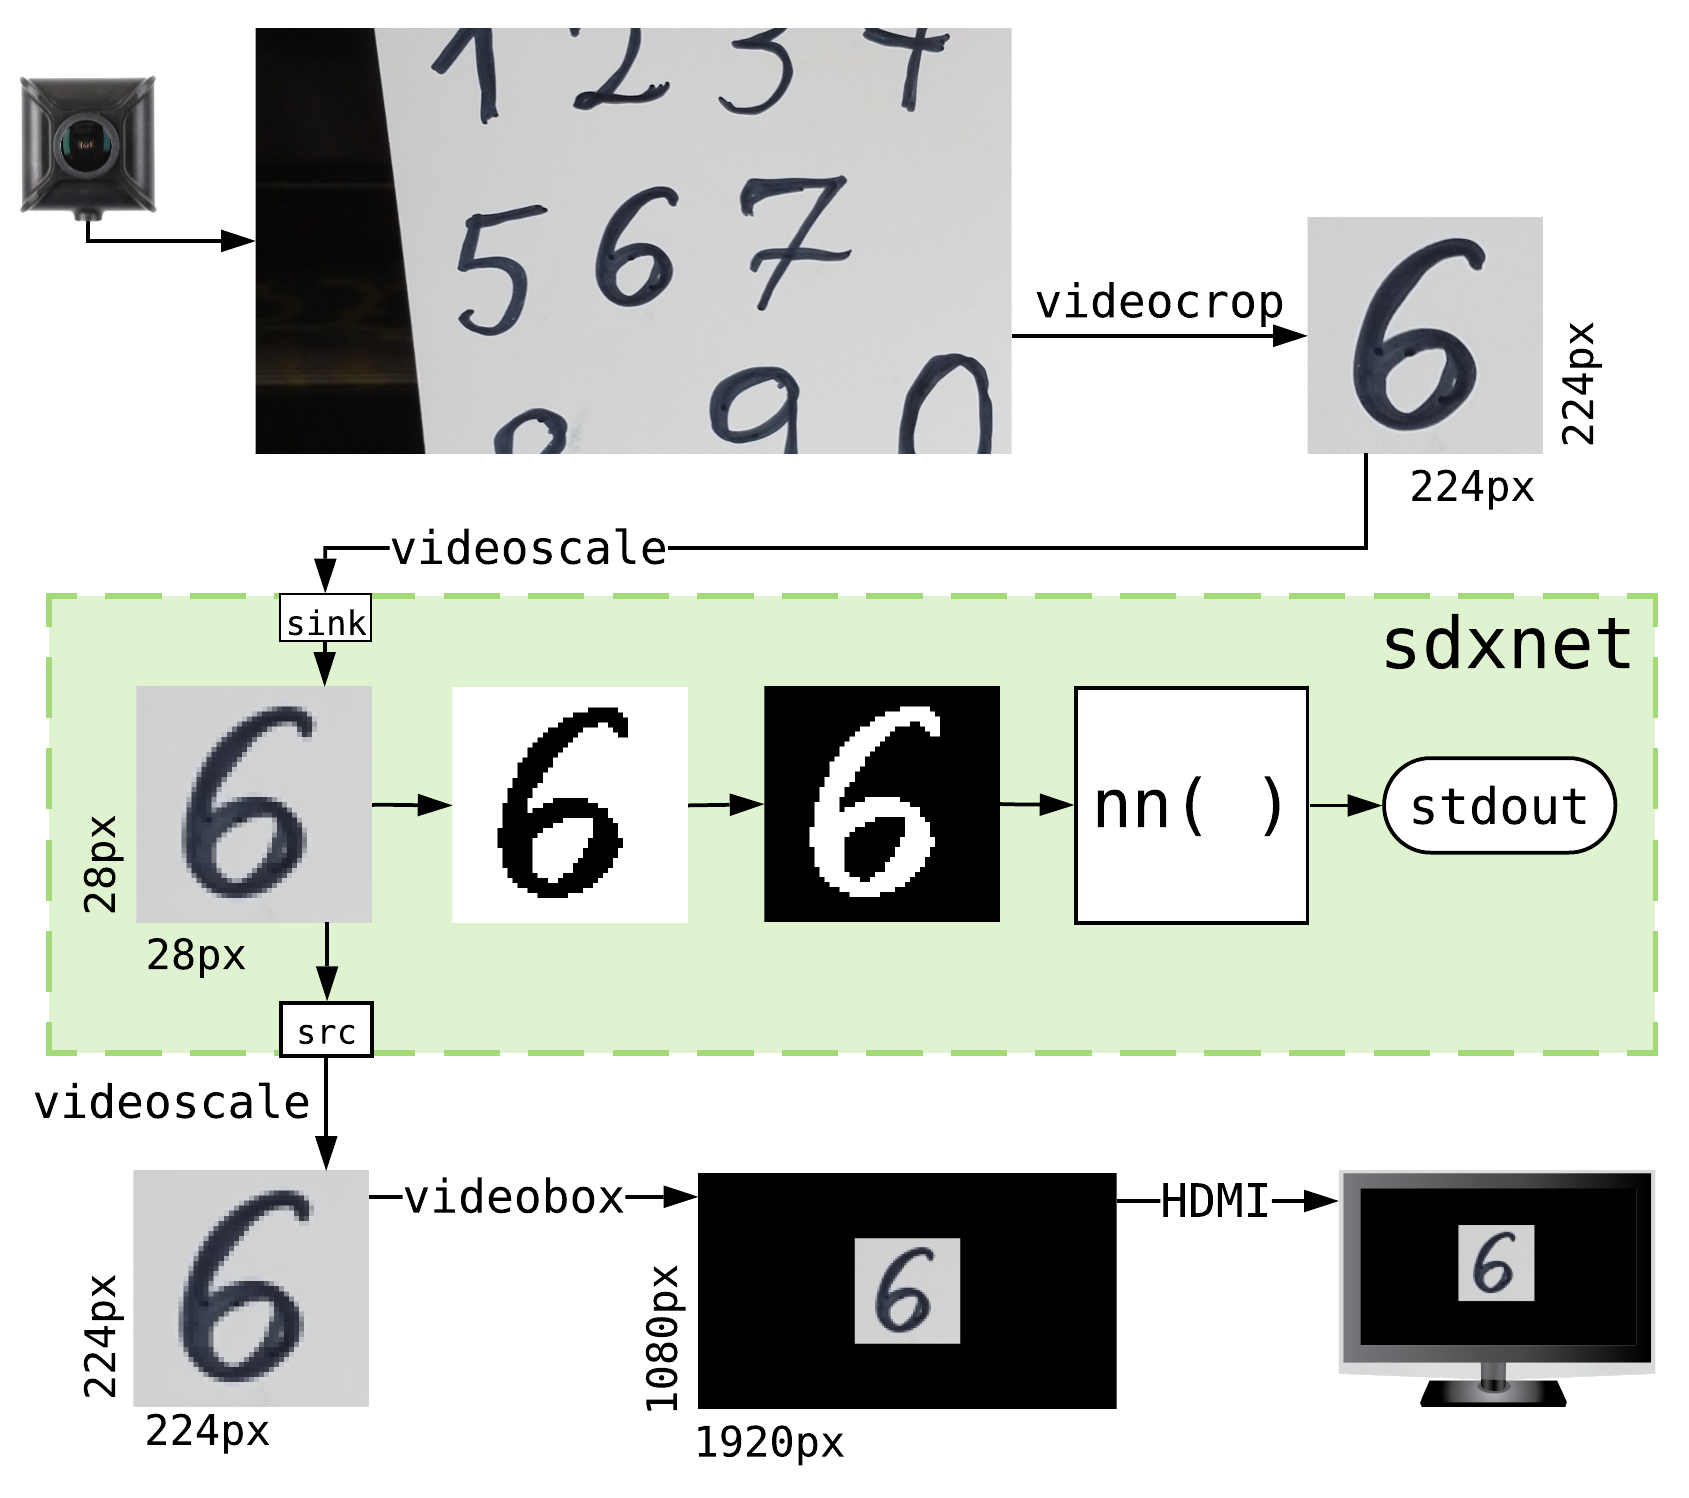
\includegraphics[width=0.95\linewidth]{figures/image_flow.png}
  \caption{Schemat logiczny przetwarzania obrazu}\label{fig:image_flow}
\end{figure}

Zsyntetyzowana sieć jest częścią projektu. Potrzebne jest również dostarczenie
danych do sieci oraz przedstawienie wyniku.
Do tego celu skorzystano z~frameworka GStreamer, dzięki któremu można
tworzyć grafy z~komponentów (pluginów, elementów)
przetwarzających media, zarówno audio jak i~video.
Każdy z~elementów grafu składa się z~co najmniej jednego źródła (source),
lub ujścia (sink), może mieć również wiele wejść i~wyjść. W~grafie pierwszy
element nie może mieć wejść, natomiast konieczne jest aby posiadał co najmniej
jedno wyjście. Poprawnie przygotowany graf nie powinien mieć komponentów
oferujących źródło, które nie są z~niczym połączone.
Pluginy mają ujednolicony interfejs, dzięki czemu można w~łatwy sposób
włączyć do grafu własny element. Wtyczki charakteryzują się
pewnymi własnościami, znanymi jako „caps”. Określają one jakie 
media jest w~stanie przetworzyć dana wtyczka (na przykład format pikseli,
maksymalny rozmiar obrazu). 
Łączone ze sobą elementy dokonują negocjacji
parametrów mediów, takich jak rozdzielczość obrazu, format pikseli,
ilość klatek na sekundę oraz innych. Wszystkie wtyczki wypisane niżej
(poza xlnxvideosink, xlnxvideosrc od Xilinx oraz sdxnet, będącego
własną implementacją) są dostępne wraz z~instalacją GStreamera.

\subsubsection{xlnxvideosrc i~xlnxvideosink}\label{sec:xlnxvideosrc i~xlnxvideosink}
Są to pluginy dostarczone przez firmę Xilinx wraz z~platformą reVISION.
Obydwa korzystają biblioteki Xilinx \lstinline{video_lib}.
Pierwszy z~nich ułatwia odczytywanie danych ze źródeł, dla których potrzebne
byłyby dodatkowe działania. Są to między innymi kamera USB (użyta w~projekcie),
HDMI, MIPI CSI (sprzętowy interfejs do transmisji obrazów i~wideo).
Sam element zbudowany jest w~oparciu o~element v4l2src\cite[s.33]{ug1221}, dostępny
w~standardowej instalacji GStreamera.
Xlnxvideosink również jest oparty o~inny element --- kmssink\cite[s.33]{ug1221}.
Zapewnia odpowiednią konfigurację połączenia z~wyświetlaczami
podłączonymi przez HDMI oraz DisplayPort.

\begin{figure}[h]
  \centering
  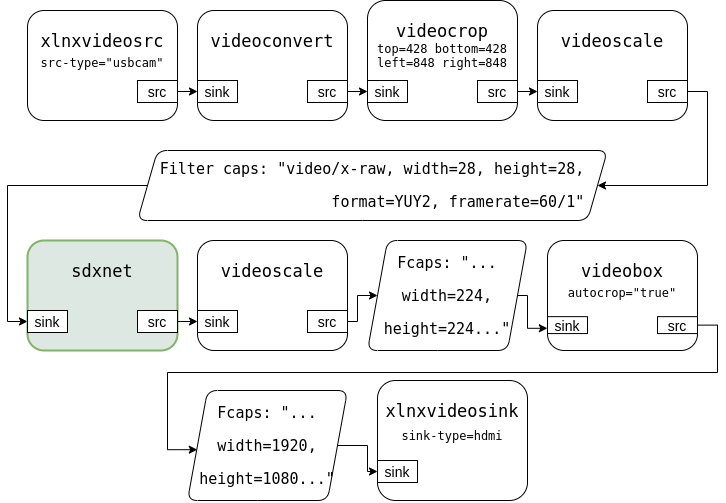
\includegraphics[width=0.9\linewidth]{figures/pipeline.png}
  \caption{Schemat grafu. Na zielono plugin z~siecią neuronową}\label{fig:pipeline}
\end{figure}

\subsubsection{videoconvert}\label{sec:videoconvert}
Element mający za zadanie dostosować wszystkie parametry obrazu tak,
aby móc połączyć ze sobą dwa niekompatybilne pod względem „caps” elementy.
Ta niekompatybilność może być spowodowana na przykład tym, że dwie
wtyczki potrzebują innego formatu pikseli i~jednocześnie nie oferują
możliwości konwersji z~jednego formatu na inny.

\subsubsection{videocrop}\label{sec:videocrop}
Wtyczka służąca do wykadrowania obrazu w~zdefiniowanym obszarze.
Wykorzystana została aby otrzymać obraz o~tej samej długości
i szerokości wynoszącej 224 (co jest ośmiokrotnością 28, czyli
długością boku obrazów, którymi wytrenowana została sieć) wycięty
ze środka wideo o~rozmiarze 1920\(\times \)1080.

\subsubsection{videoscale}\label{sec:videoscale}
Skaluje obraz do wynegocjowanych pomiędzy sąsiadującymi elementami
parametrów, przy czym pierwsza próba negocjacji to ta sama wielkość
obrazu przy ujściu jak i~w~źródle, aby skalowanie nie było potrzebne.

\subsubsection{sdxnet}\label{sec:sdxnet}
Sdxnet to wtyczka wykorzystująca sieć neuronową do rozpoznania cyfr
znajdujących się na obrazie przez nią przechodzącym. Element ten został
zaimplementowany na potrzeby tego projektu.

\subsubsection{Filter caps}\label{sec:Filter caps}
Element precyzujący parametry obrazu, które wymuszają
dostosowanie się poprzedniego elementu --- na przykład videoscale.
Zapisuje się go w~postaci ciągu znaków ujętych w~cudzysłów.

\subsubsection{videobox}\label{sec:videobox}
Oferuje możliwość osadzenia obrazu w~tym o~innym
rozmiarze wypełniając pozostałą przestrzeń ramką
w wybranym kolorze. Własność autocrop oznacza automatyczne obliczenie
wielkości ramek na podstawie parametrów określonych przez kolejny element tak,
aby obraz przychodzący do videobox był wycentrowany a~ramki
były tej samej wielkości.

\subsubsection{fpsdisplaysink}\label{sec:fpsdisplaysink}
Wtyczka typu sink (mająca tylko ujście), która jako parametr
pobiera inną wtyczkę tego typu, np.~xlnxvideosink,
zastępując w~grafie tamtą.
Jej użycie pozwala na sprawdzenie liczby klatek na sekundę
wyświetlanego obrazu.


\subsection{Używanie sieci}\label{sec:Uzywanie sieci}
\subsubsection{Generowanie projektu}\label{sec:Generowanie projektu}
Architekturę sieci wraz z~wagami zapisano do pliku h5. Stworzono
plik konfiguracyjny hls4ml. Następnie na jego podstawie wygenerowano projekt
z przekonwertowaną siecią. Wśród wygenerowanych plików znajduje się
również kod służący do symulacji działania projektu. Przygotowane zostały
pliki z~danymi testującymi sieć --- 10000 przetworzonych przykładów z~bazy
MNIST tak, aby cyfry były koloru czarnego, tło białego. Zakres wartości
wynosi od 0 do 255.

\subsubsection{Funkcja}\label{section:funkcja}
Cała sieć jest przedstawiona jako jedna funkcja o~nazwie \lstinline{nn}.
Parametrami tej funkcji są dwie tablice:
\lstinline[style=hls]{input[]}, do której są zapisywane są
dane do przetworzenia,
oraz \lstinline[style=hls]{output[]}, do której funkcja zapisuje
obliczone predykcje.

\begin{minipage}{\linewidth}
\lstinputlisting[
  caption={Nagłówek funkcji},
  label={lst:nn_header},
  style=hls
]{listings/nn.h}
\end{minipage}

\subsubsection{Interfejs}\label{sec:Interfejs}
Aby móc korzystać z~sieci w~aplikacji uruchamianej na procesorze ARM
zadeklarowano użycie interfejsu IO \mbox{AXI-4} Lite.

\subsubsection{Dostosowanie sieci}\label{sec:Dostosowanie sieci}
W celu poprawienia wyników działania sieci dokonano pewnych usprawnień.
Sieć została wytrenowana oryginalnymi danymi, w~których piksele tworzące
cyfry mają wartości równe 255 lub tej wartości bliskie,
a piksele białego są przedtawione jako 0.
Ponadto rzeczywiste dane z~kamery mogą być zaszumione,
przedstawione obiekty zacienione, a~same cyfry mogą nie być idealnie czarne.

Przy każdym wywołaniu funkcji sieci dokonywana jest transformacja
danych poprzez kod pokazany na listingu~\ref{lst:data_tresh}.
Wartość każdego piksela jest zamieniana na wartość 255 lub 0, zależnie
od początkowej jego wartości --- dla wartości mniejszych od 140
(kolor szary lub ciemniejszy) przypisany jest kolor biały, wartość 255.
Dla pikseli jasnych (od 140 w~górę) przypisywana wartość to 0, kolor czarny.

W ten sposób dokonuje się zarówno odpowiedniego przetworzenia danych
uwzględniającego sposób wytrenowania modelu, jak również uwydatnienia
cyfry oraz pozbycia się szumów obrazu i~jasnych cieni.

\hspace{-1cm}
\begin{minipage}{\linewidth}
\lstinputlisting[
  caption={Transformacja danych.},
  label={lst:data_tresh},
  firstline=36,
  lastline=39,
  language=C++
  % floatplacement=H
]{listings/nn.cpp}
\begin{itemize}
  \setlength{\itemindent}{3em}
  \item \lstinline[style=hls]{input[]} --- tablica z~danymi (parametr funkcji)
  \item \lstinline[style=hls]{input1[]} --- dane przetwarzane przez sieć
\end{itemize}
\end{minipage}

% \newpage
\subsubsection{Tworzenie biblioteki}\label{section:create_library}

Zsyntetyzowany moduł sieci został wyeksportowany w~środowisku Vivado HLS
do paczki IP (Intelectual Property). Następnie poprzez narzędzie
\lstinline{sdx_pack} utworzono statyczną bibliotekę gotową do wykorzystania
w innym projekcie w~środowisku SDSoC (Software-Defined System on Chip,
IDE do pisania aplikacji lub bibliotek uruchamianych na platformach
Xilinx MPSoC).

Wywołując narzędzie \lstinline{sdx_pack} należy podać plik nagłówkowy funkcji,
docelową nazwę biblioteki,
ścieżkę do pliku \lstinline{component.xml} wygenerowanego podczas eksportu
do paczki IP, mapowanie parametrów funkcji na porty modułu,
protokół kontroli modułu, odpowiedni zegar oraz informacje
dotyczące docelowej platformy: nazwę jej rodziny, procesora oraz systemu.

\hspace{1mm}
\begin{minipage}{0.95\linewidth}
\lstinputlisting[
  caption={Narzędzie sdx\_pack},
  label={lst:sdx_pack},
]{listings/sdx_pack.sh}
\end{minipage}

\begin{figure}[h]
  \centering
  \includesvg[width=0.92\linewidth]{figures/sdx_pack-scheme}
  \caption{Schemat tworzenia biblioteki \\
  Za \textit{SDSoC Environment User Guide: C-Callable IP Libraries},
  \url{https://china.xilinx.com/html_docs/xilinx2018_3/sdsoc_doc/c-callable-libraries-zah1504034388097.html}}\label{fig:ccallable}
\end{figure}

\newpage
\subsection{Implementacja pluginu sdxnet}\label{sec:Implementacja pluginu sdxnet}

% \begin{figure}
%   \centering
%   \includegraphics[width=\linewidth,
%     trim={3cm 4cm 2.5cm 3cm}, clip]
%   {figures/kod-scheme.pdf}
%   \caption{Schemat przetwarzania danych}\label{fig:code-scheme}
% \end{figure}
Dalsza część implementacji składa się z~dwóch części.
Pierwsza z~nich to \lstinline{neuralnet}, biblioteka statyczna, która
odpowiada za inicjalizację i~zwolnienie pamięci dla danych, z~których
korzystają funkcje akcelerowane sprzętowo,
wyciągnięcie danych dotyczących luminacji z~obrazu,
wywołanie funkcji \lstinline{nn} (patrz rozdział~\ref{section:funkcja}) oraz
za utworzenie obrazu wychodzącego z~pluginu.
Druga część to biblioteka dzielona \lstinline{gstsdxnet}, korzystająca
z~funkcji z~biblioteki \lstinline{neuralnet}. Biblioteka ta jest rozpoznawana
jako plugin GStreamer, można więc z~niej korzystać przy budowaniu
grafów za pomocą GStreamera. Schemat wykonywania kodu przedstawiony jest
na stronie~\pageref{appendix:code-scheme}.

\subsubsection{neuralnet}\label{sec:neuralnet}
Dane obrazu (kanał luminacji i~kanał chrominacji)
przechowywane są w~obiektach klasy \lstinline{xf::Mat} będącej
częścią bibliotek xfOpenCV. Określona jest wysokość oraz szerokość obrazu,
typ pikseli kodujących obraz (w~tym przypadku ośmiobitowe bez znaku
z~jednym kanałem pikseli). Pamięć dla tych obiektów oraz dla tablicy
przechowującej predykcje sieci alokowana jest przez
funkcję \lstinline{net_init_sds}, a~zwalniana przez funkcję
\lstinline{net_deinit_sds}. Dla każdej klatki obrazu z~poziomu
\lstinline{gstsdxnet} wywoływane są kolejno trzy funkcje:
\lstinline{net_sds_read},
\lstinline{net_sds_predict} oraz
\lstinline{net_sds_write}.

Pierwsza z~nich rozkodowuje przy pomocy masek i~przesunięć bitowych
dane z~pikseli i~zapisuje je do dwóch kanałów (obiektów \lstinline{xf::Mat}).
Ostatnia, również używając tych samych bitowych operacji, łączy obydwa kanały
tworząc wyjściowy obraz, przy czym dla kanału luminacji są to dokładnie te
same dane, które zostały odczytane przez \lstinline{net_sds_read},
natomiast wszystkie bajty kanału chrominacji mają wartość 128,
aby wyjściowy obraz był w~skali szarości (dzięki czemu
obraz na monitorze jest bardziej zbliżony do tego rzeczywiście przetwarzanego).
Obydwie funkcje korzystają z~funkcji akcelerowanych
sprzętowo aby zrównoleglić i przyspieszyć w~ten sposób proces.
Funkcja \lstinline{net_sds_predict} wywołuje funkcję \lstinline{nn} oraz
kopiuje otrzymane predykcje do tablicy otrzymanej z~\lstinline{gstsdxnet}.

Przy kompilacji biblioteki należy dołączyć bibliotekę statyczną
powstałą w~procesie opisanym w~rozdziale~\ref{section:create_library}.

\subsubsection{gstsdxnet}\label{sec:gstsdxnet}
Framework GStreamer jest w~stanie rozpoznać bibliotekę \lstinline{gstsdxnet}
dzięki napisaniu funkcji spełniających wymagania stawiane przez framework.
Obejmują one inicjalizację pluginu (m.in.~alokacja pamięci, zdefiniowanie
możliwych parametrów mediów na wejściu i~na wyjściu, zapisanie
metadanych), funkcję
przetwarzającą klatki obrazu oraz te odpowiadające za prawidłowe zakończenie
pracy wtyczki. Funkcja inicjalizująca plugin uruchamia też funkcję
inicjalizującą z~biblioteki \lstinline{neuralnet}.
Funkcja przetwarzająca obraz (\lstinline{gst_sdx_process_frames}
przygotowuje dane, które przekazuje do
odpowiednich funkcji z~\lstinline{neuralnet}. Dla co dwudziestej piątej
klatki obrazu na standardowe wyjście zapisywany jest wynik predykcji
w postaci pary liczb (przewidywana cyfra, prawdopodobieństwo). 

Kod wtyczki oparto o~kod przykładowej wtyczki dostarczonej wraz
z platformą reVISION \mbox{2018-3} przez Xilinx.

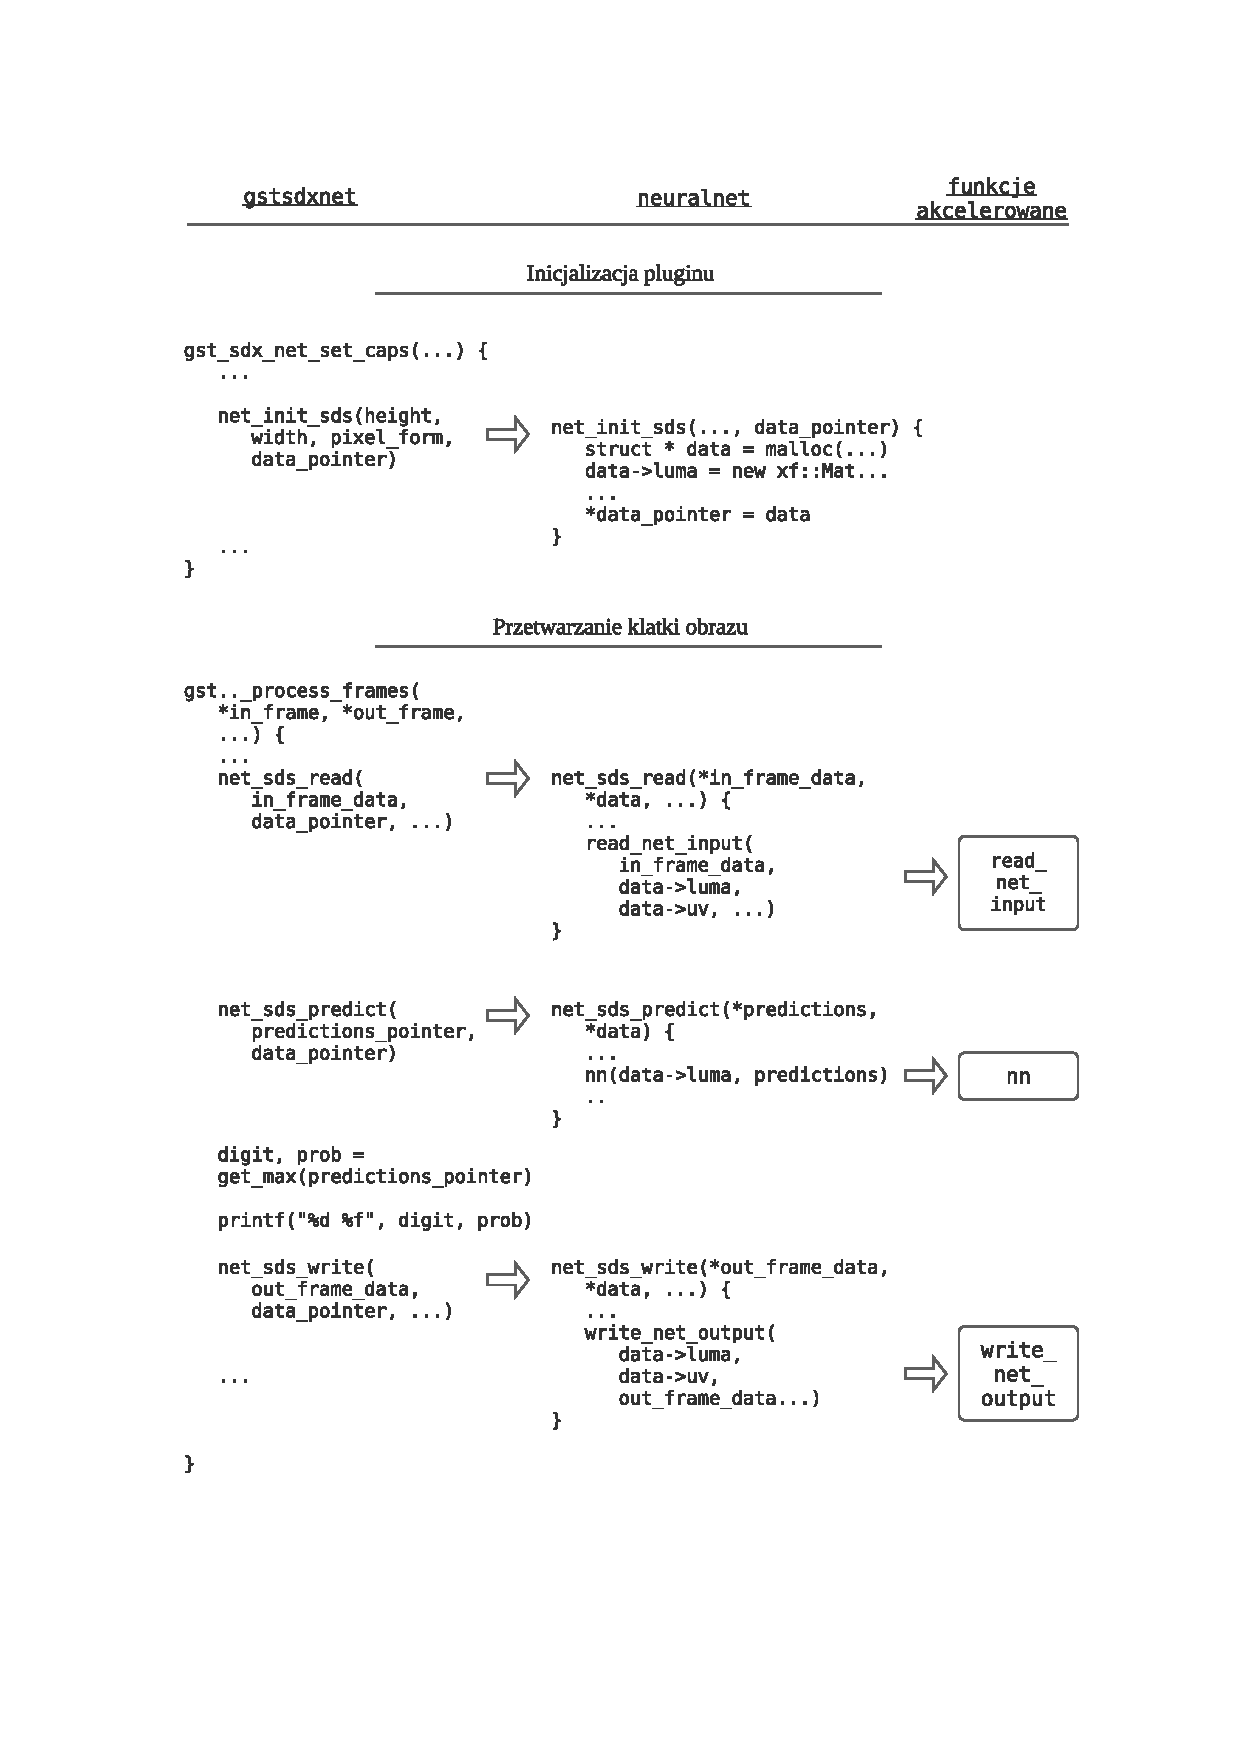
\includepdf[pagecommand={}\label{appendix:code-scheme}]{figures/kod-scheme.pdf}

\newpage
\subsection{Uruchamianie}\label{sec:Uruchamianie}
Aby uruchomić pipeline przedstawiony na rysunku~\ref{fig:pipeline}
można skorzystać z~narzędzia \lstinline{gst-launch-1.0}.
Narzędzie ułatwia i~przyspiesza uruchamianie różnych strumieni
przetwarzających media, ponieważ nie ma potrzeby zaprogramowania
aplikacji. Narzędzie jako argumenty wywołania programu pobiera
nazwy pluginów oddzielone znakiem wykrzyknika
w~kolejności w~jakiej mają wystąpić w~grafie. Skrypt przedstawiono
na listingu~\ref{lst:script} na stronie~\pageref{lst:script}.

\begin{figure}[h]
  \centering
  \includesvg[width=0.9\linewidth]{figures/physical-scheme.svg}
  \caption{Uproszczony schemat przedstawiający działanie
  projektu na sprzęcie.
  Czarnymi strzałkami oznaczono pomiędzy jakimi elementami
  następuje wymiana danych, na czerwono kontrolę procesora}\label{fig:physical-scheme}
\end{figure}

\newpage
% \hspace{1cm}
\begin{minipage}{\linewidth}
\lstinputlisting[
  caption={Skrypt uruchamiający cały projekt},
  label={lst:script},
  showstringspaces=false
]{listings/script.sh}
\end{minipage}


\newpage
\section{Wyniki i~dyskusja}\label{sec:Wyniki i~dyskusja}
W~tym rozdziale przedstawione są wyniki prezentujące dokładność
predykcji dokonywanych przez model na różnych etapach implementacji
projektu zaczynając od testach w~Pythonie, a~kończąc na sprawdzeniu
działania w~pełni zaimplementowanego projektu.

\subsection{Ewaulacja modelu}\label{sec:Ewaulacja modelu}
Do testów w~Pythonie użyto 10000 próbek z~bazy MNIST, którymi nie
wytrenowano modelu. Osiągnięta dokładność wynosi 92,22\%. 

\subsection{Symulacja}\label{sec:Symulacja}
Kolejne testy przeprowadzono po konwersji modelu sieci do kodu \CPP{}
przez hls4ml. Danymi testowymi były te same próbki z~bazy MNIST.
Liczba dobrze sklasyfikowanych cyfr spadła --- osiągnięto 90,52\%
dokładności.

\subsection{Dane rzeczywiste}\label{sec:Dane rzeczywiste}
Kompletny projekt przetestowano na zbiorze liczącym 20 cyfr (patrz
rys.~\ref{fig:test_data}). Cyfry
zapisano odręcznie czarnym markerem na białym papierze. Dla każdej z~nich
dokonano pomiarów, a~uzyskane wyniki zapisano w~tabeli~\ref{tab:results}.

\begin{figure}[h]
  \centering
  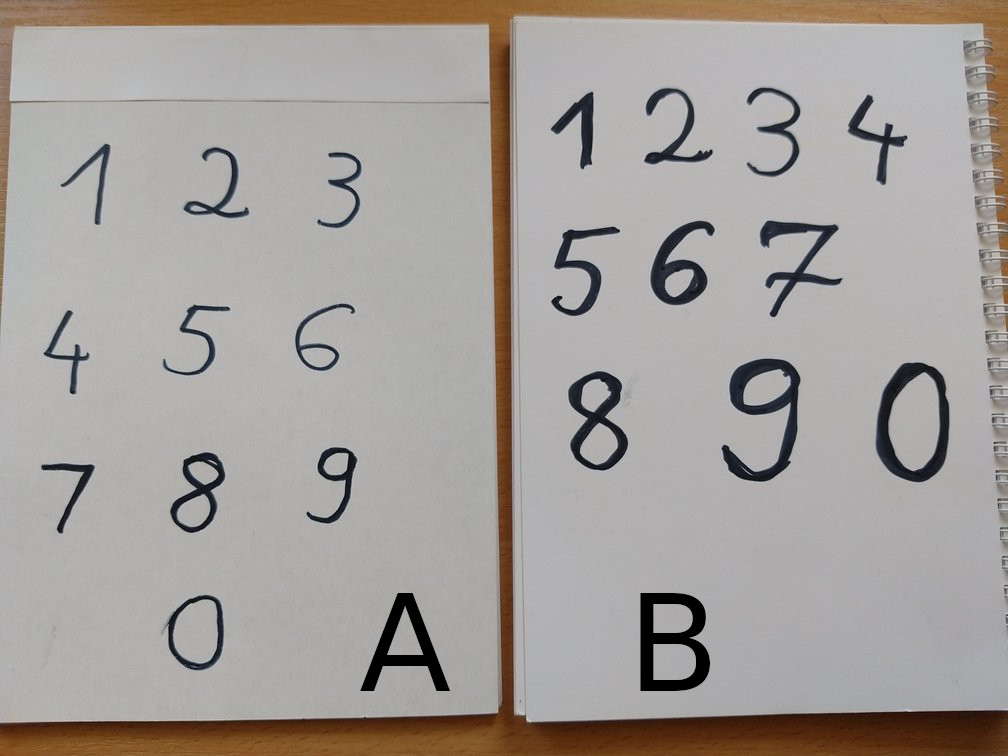
\includegraphics[width=0.9\linewidth]{figures/test_data.jpg}
  \caption{Przygotowane zestawy danych testowych}\label{fig:test_data}
\end{figure}


\subsubsection{Tabela z~wynikami}\label{sec:Tabela z~wynikami}
Dla każdej z~cyfr wykonano kilkadziesiąt odczytów. W~tabeli~\ref{tab:results}
podane są najistotniejsze z~nich.
Pierwsza kolumna oznacza rzeczywistą cyfrę. W~kolumnach „zestaw A” i~„zestaw B”
podane wyniki dla cyfr z~zestawów przedstawionych
na rysunku~\ref{fig:test_data}.
Każda komórka zawiera maksymalną odczytaną wartość prawdopodobieństwa
przynależności do danej klasy (lub „nie rozpoznano” jeśli sieć ani razu
nie rozpoznała poprawnie cyfry)
oraz wszystkie wystąpienia błędnych predykcji wraz z~odpowiadającym im
największymi odczytami prawdopodobieństwa (o ile takie wystąpiły).
Ze względu na użyty typ danych w~ostatniej warstwie sieci
wyniki otrzymano z~dokładnością do 6,25 punkta procentowego.

\begin{table}[h]
\centering
\begin{tabular}{ r r r }
  Cyfra & zestaw A & zestaw B \\ [0.5ex]
  \toprule 
  0  
  & 97,5\%
  & \begin{tabular}{@{}r@{}r@{}}97,5\% \\ „3” 67,5\% \\ „2” 62,5\% \end{tabular}
    \\ \midrule
  1  
  & \begin{tabular}{@{}r@{}}nie rozpoznano\\ „7” 81,25\% \end{tabular}
  & \begin{tabular}{@{}r@{}}92,5\% \\ „7” 62,5\% \end{tabular}
    \\ \midrule
  2
  & \begin{tabular}{@{}r@{}}100\% \\ „3” 50\% \end{tabular}
  & 100\%
    \\ \midrule
  3
  & 100\%
  & 100\%
    \\ \midrule
  4
  & \begin{tabular}{@{}r@{}}92,5\% \\ „9” 92,5\% \end{tabular}
  & \begin{tabular}{@{}r@{}}do 37,5\% \\ różne cyfry do 60\% \end{tabular}
    \\ \midrule
  5
  & \begin{tabular}{@{}r@{}r@{}}62,5\% \\ „2” 43,75\% \\ „3” 37,5\% \end{tabular}
  & \begin{tabular}{@{}r@{}r@{}}87,5\% \\ „6” 56,25\% \\ „3” 31,25\% \end{tabular}
    \\ \midrule
  6
  & 87,5\%
  & \begin{tabular}{@{}r@{}}100\% \\ „2” 62,5\%  \end{tabular}
    \\ \midrule
  7
  & \begin{tabular}{@{}r@{}r@{}}nie rozpoznano\\ „6” 93,75\% \\ „2” 62,5\%  \end{tabular}
  & 100\%
    \\ \midrule
  8
  & 93,75\%
  & \begin{tabular}{@{}r@{}r@{}}93,75\% \\ „3” 75\% \\ „9” 43,75\%  \end{tabular}
    \\ \midrule
  9
  & \begin{tabular}{@{}r@{}r@{}}nie rozpoznano\\ „3” 93,75\% \\ „8” 87,5\%  \end{tabular}
  & \begin{tabular}{@{}r@{}r@{}}nie rozpoznano\\ „3” 87,5\% \\ „2” 56,25\%  \end{tabular}
    \\ 
  \bottomrule
\end{tabular}
  \caption{Wyniki dla danych rzeczywistych z~kamery}\label{tab:results}
\end{table}

\subsubsection{Omówienie wyników}\label{sec:omowienie_wynikow}
Dla 14 spośród 20 cyfr otrzymano wyniki z~prawdopodobieństwem wynoszącym
co najmniej 87,5\%. Dla cyfr „2” i~„3” uzyskano wiele odczytów
ze stuprocentowym prawdopodobieństwem dla obydwu zestawów. Cyfry „0”, „6” i~„8”
również były w~większości odczytów poprawnie kwalifikowane. Małe problemy
nastąpiły przy próbach odczytu cyfr „1”, „4” i~„7”, w~których sieć nie była
w stanie poprawnie określić klasy, natomiast poprawnie odczytywała tę cyfrę
z drugiego zestawu. Jedynie cyfra „9” nie została w~żadnym z~przypadków
rozpoznana, ponadto błędnie odczytywana jako cyfra „3” z~obu zestawów.

Każda próba pomiaru cyfry dawała wiele wyników w~zależności od położenia
cyfry na obrazie, jej grubości, kąta pod jakim jest nagrywana. Pomiary starano
robić się tak, aby środek cyfry pokrywał się ze środkiem obrazu, a~także
żeby cyfra nie stykała się z~jego krawędzią. Dla wszystkich próbek sprawdzano
różne odległości, przesunięcia cyfry względem środka obrazu i~kąty.
Zauważono, że przy kilku próbkach, szczególnie dla cyfry „5”,
najmniejsze poruszenie kamery
wynikające z~niestabilności ręki wpływało w~znacznym stopniu na predykcję.

\subsection{Dyskusja}\label{sec:Dyskusja}
Na każdym z~etapów implementacji można zauważyć spadek dokładności sieci.
\linebreak
Po przetłumaczeniu modelu sieci przez hls4ml jest to głównie spowodowane
zmniejszeniem precyzji danych na jakich sieć dokonuje obliczeń. 
Na ostatnim etapie spadek związany jest z~możliwymi szumami obrazu,
niewystarczająco dobrym nakierowaniem kamery na cyfrę, złym oświetleniem lub
innymi zewnętrznymi przyczynami. Sieć o~tej stosunkowo małej architekturze
może mieć problem z~rozpoznawaniem cyfr o~takim kształcie i~położeniu
na obrazie, z~którym nie miała do czynienia w~trakcie trenowania.
Możliwym rozwiązaniem tych problemów mogłoby być zastosowanie sieci
splotowej (konwolucyjnej), na przykład \mbox{LeNet-5}, która nie tylko
osiąga zdecydowanie wyższy wynik w~trakcie ewaluacji ale również lepiej
radzi sobie z~generalizowaniem kształtów znajdujących się na obrazie.
W przeprowadzonym teście architektury \mbox{LeNet-5} osiągnięto wynik
99,18\% dobrze rozpoznanych cyfr, jednak z~wcześniej
wspomnianych powodów nie wykorzystano takiej architektury.


\newpage
\newgeometry{top=3cm, left=2.5cm, right=2.5cm}
\section*{Podsumowanie}
\addcontentsline{toc}{section}{Podsumowanie}%
Celem pracy był projekt, który pozwala na
rozpoznawanie cyfr w~czasie rzeczywistym, korzystając z~modelu sieci
neuronowej zaimplementowanej na układzie FPGA. Całość można określić jako
GStreamer pipeline, spośród którego elementów można wyróżnić wtyczkę
do rozpoznawania cyfr, korzystającą z~sieci neuronowej, wtyczki odpowiadające
za wstępne przetworzenie obrazu oraz te, które umożliwiają wyświetlenie obrazu
na urządzeniu zewnętrznym.

W rozdziale~\ref{sec:Teoria} została przedstawiona teoria przydatna
do zrozumienia projektu. Opisana została architektura FPGA
w~rozdziale~\ref{sec:Architektura FPGA}, informacje o~przetwarzaniu
obrazu (\ref{sec:Przetwarzanie obrazu}) w~tym opis użytego formatu pikseli
oraz krótki opis jak działają sieci neuronowe (\ref{sec:Sieci neuronowe}).

Przedstawiono również sam projekt zaczynając od ogólnego
zarysu (\ref{sec:Zarys projektu}), pokazania platformy z~której korzystano
(\ref{sec:Platforma}) i~prezentacji architektury sieci (\ref{sec:Siec neuronowa}).
Następnie przybliżono frameworki hls4ml (\ref{sec:hls4ml})
i GStreamer (\ref{sec:GStreamer}). Został opisany i~przedstawiony
również sam GStreamer pipeline
w~rozdziałach~\ref{sec:xlnxvideosrc i~xlnxvideosink}--\ref{sec:fpsdisplaysink}.

Przybliżony został proces implementacji modelu sieci na FPGA
w~rozdziale~\ref{sec:Uzywanie sieci}, gdzie opisano jak dostosować kod będący
wynikiem działania hls4ml do poprawnego działania z~resztą projektu
oraz w~jaki sposób utworzyć z~niej bibliotekę dzieloną, z~której można
korzystać w~projektach SDSoC.

Ostatnie podrozdziały rozdziału~\ref{sec:Opis projektu} dotyczą
wykorzystania utworzonej biblioteki dzielonej w~implementacji wtyczki
GStreamer. Proces tworzenia został podzielony na dwie części (neuralnet,
patrz~\ref{sec:neuralnet} i~gstsdxnet --- \ref{sec:gstsdxnet}), aby
w~logiczny sposób oddzielić od siebie potrzebne funkcjonalności.

Na samym końcu zaprezentowano otrzymane wyniki na różnych etapach
implementacji sieci neuronowej: jako model w~Pythonie, w~trakcie symulacji
komputerowej przed syntezą oraz po pełnej implementacji, wykorzystując
własne dane testowe (patrz rys.~\ref{fig:test_data}).

W implementacji projektu jest wiele rzeczy, które można poprawić lub
w jakiś sposób ulepszyć. Wśród nich jest wykorzystanie innej architektury
sieci, aby otrzymać większą skuteczność rozpoznawania cyfr, przeniesienie
części odpowiedzialnej za wstępne przetworzenie obrazu do funkcji
akcelerowanych sprzętowo w~celu poprawienia wydajności, inny sposób
prezentacji wyniku, na przykład na wyświetlanym obrazie, kończąc
na samym sposobie informowania użytkownika jaka część obrazu będzie
klasyfikowana przez sieć --- wizualne oznaczenie fragmentu obrazu zamiast
wykadrowania reszty. Na wszystkie wyżej
wymienione poprawy zabrakło czasu, możliwości
sprzętowych lub wiedzy dotyczącej platformy reVISION.

W~repozytorium BitBucket\cite{repozytorium} udostępnione zostały pliki źródłowe
pozwalając na odtworzenie projektu. Udostępniono również stosowne instrukcje.

\restoregeometry{}

\begin{thebibliography}{9}
  \raggedright{}

  \bibitem{kuon08}
    I. Kuon, R. Tessier i J. Rose,
    \emph{FPGA Architecture: Survey and Challenges, Foundations
    and Trends\textregistered{} in Electronics Design Automation}.
    Tom 2,
    2007

  \bibitem{revision}
    Xilinx,
    platforma reVISION w repozytorium GitHub \linebreak
    \url{https://github.com/Xilinx/Embedded-Reference-Platforms-User-Guide/blob/2018.3/README.md}
    (dostęp 18.08.2020)
    
  \bibitem{lecun98}
  Y. LeCun, L. Bottou, Y. Bengio, P. Haffner,
  \emph{Gradient-Based Learning Applied to Document Recognition}.
  1998

  \bibitem{mnist}
  Y. LeCun, C. Cortes, C. Burges,
  Baza danych MNIST
  \url{http://yann.lecun.com/exdb/mnist/}
  (dostęp 18.08.2020)

  \bibitem{ug1221}
  Xilinx,
  \emph{Zynq UltraScale+ MPSoC Base Targeted Reference Design, User Guide}.
  UG1221 (v2018.3),
  2018

  \bibitem{repozytorium}
  \emph{Repozytorium NN-Revision na BitBucket z plikami źródłowymi} \linebreak
  \url{https://bitbucket.org/fpgafais/nn-revision/src/master/}
  (dostęp 20.08.2020)
  
\end{thebibliography}

\end{document}